% Figures

% ranked improvement - FULL
\begin{figure}
    \centering
    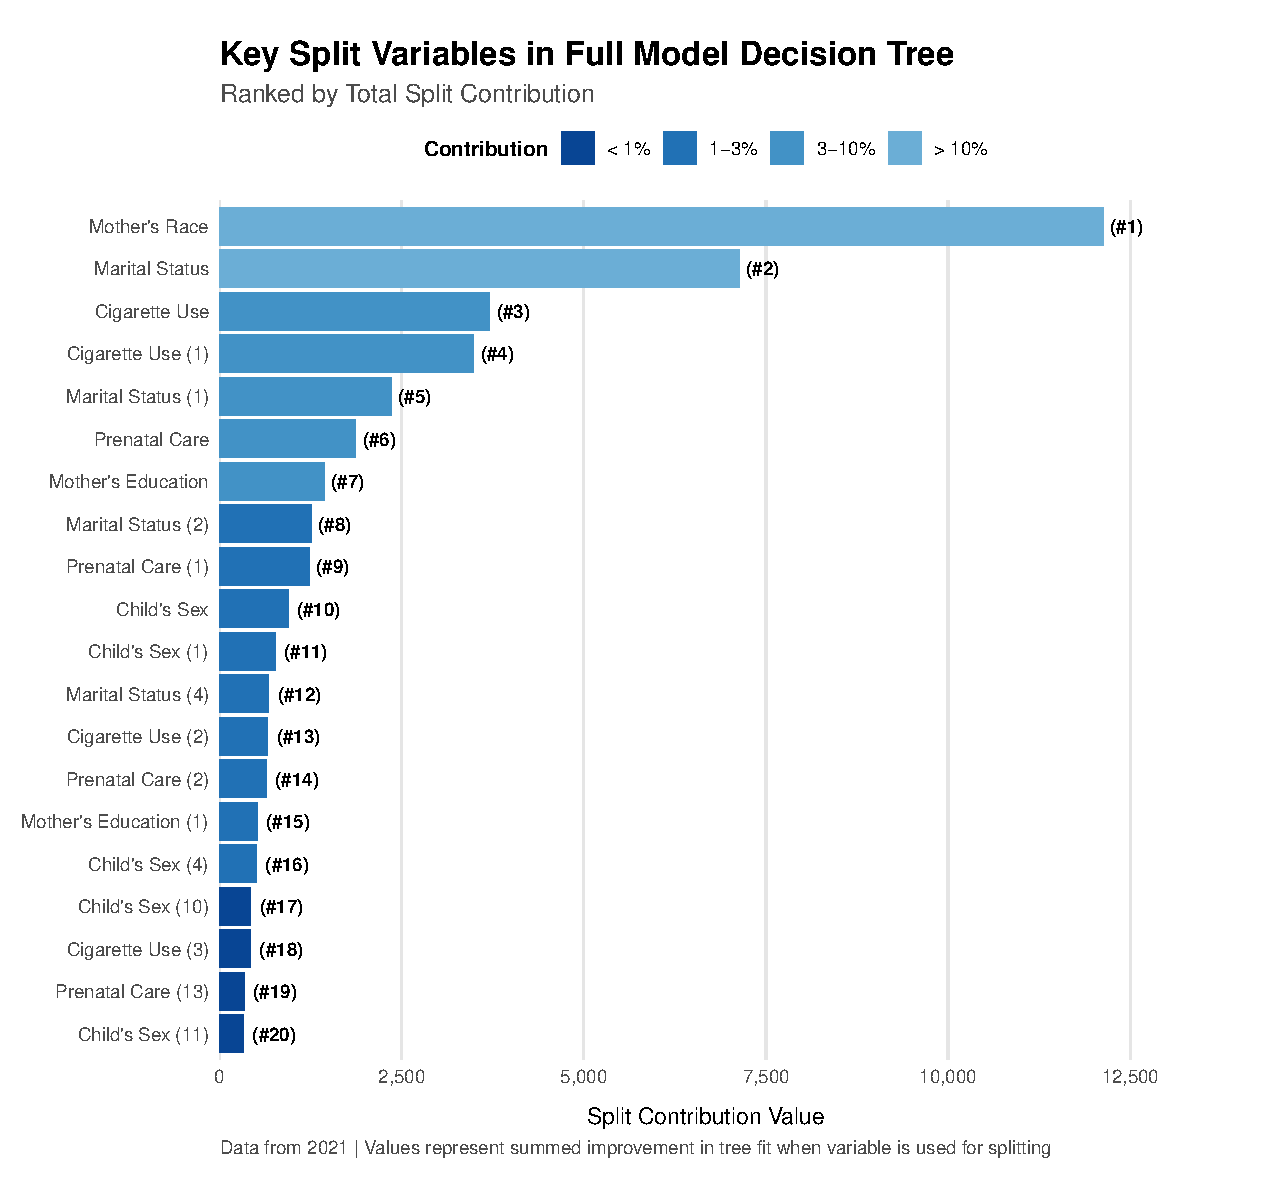
\includegraphics[width=1\linewidth]{chapters/chapter3/figures/improvement/tree_split_contribution_top20_Full Model.pdf}
    \caption{Full Model Ranked Improvement. Rankings represent summed reduction in deviance (improvement in model fit) across all nodes where each variable is used for splitting in the tree. Plot only displays top 20 ranked variables.}
    \label{fig:full-model-ranked-imp}
\end{figure}

% ranked improvement - LBW
\begin{figure}
    \centering
    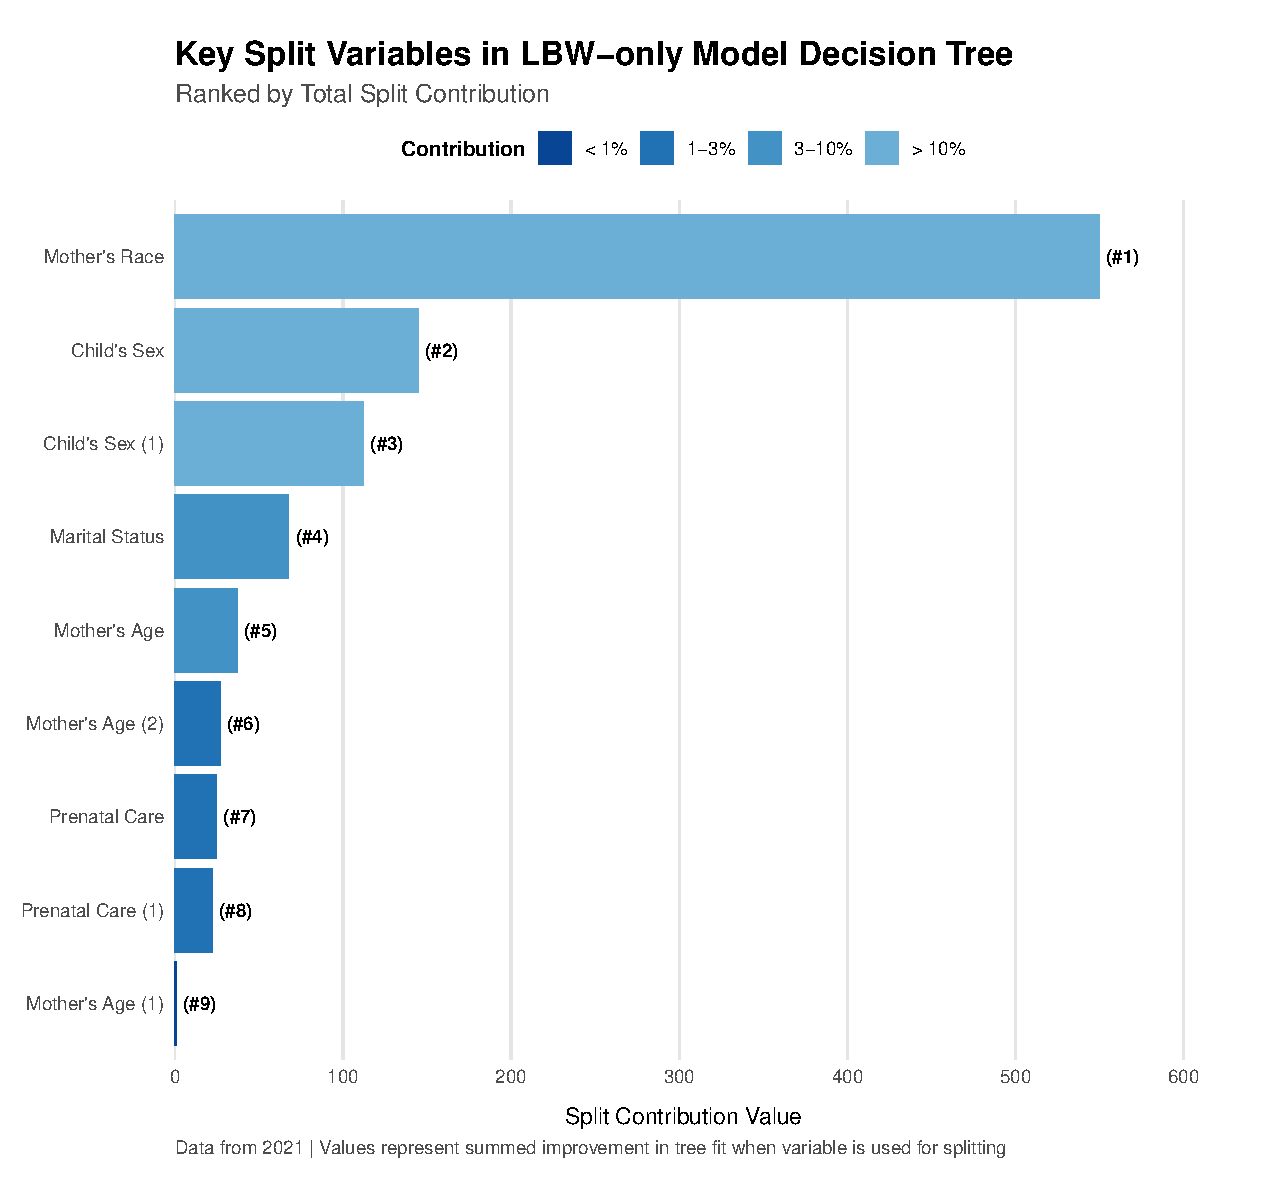
\includegraphics[width=1\linewidth]{chapters/chapter3/figures/improvement/tree_split_contribution_top9_LBW-only Model.pdf}
    \caption{LBW-only Model Ranked Improvement. Rankings represent summed reduction in deviance (improvement in model fit) across all nodes where each variable is used for splitting in the tree. Plot displays all ranked variables.}
    \label{fig:lbw-model-ranked-imp}
\end{figure}

% depth comparison - FULL
\begin{figure}[p]
    \centering
    % First row
    \begin{minipage}{0.48\textwidth}
        \centering
        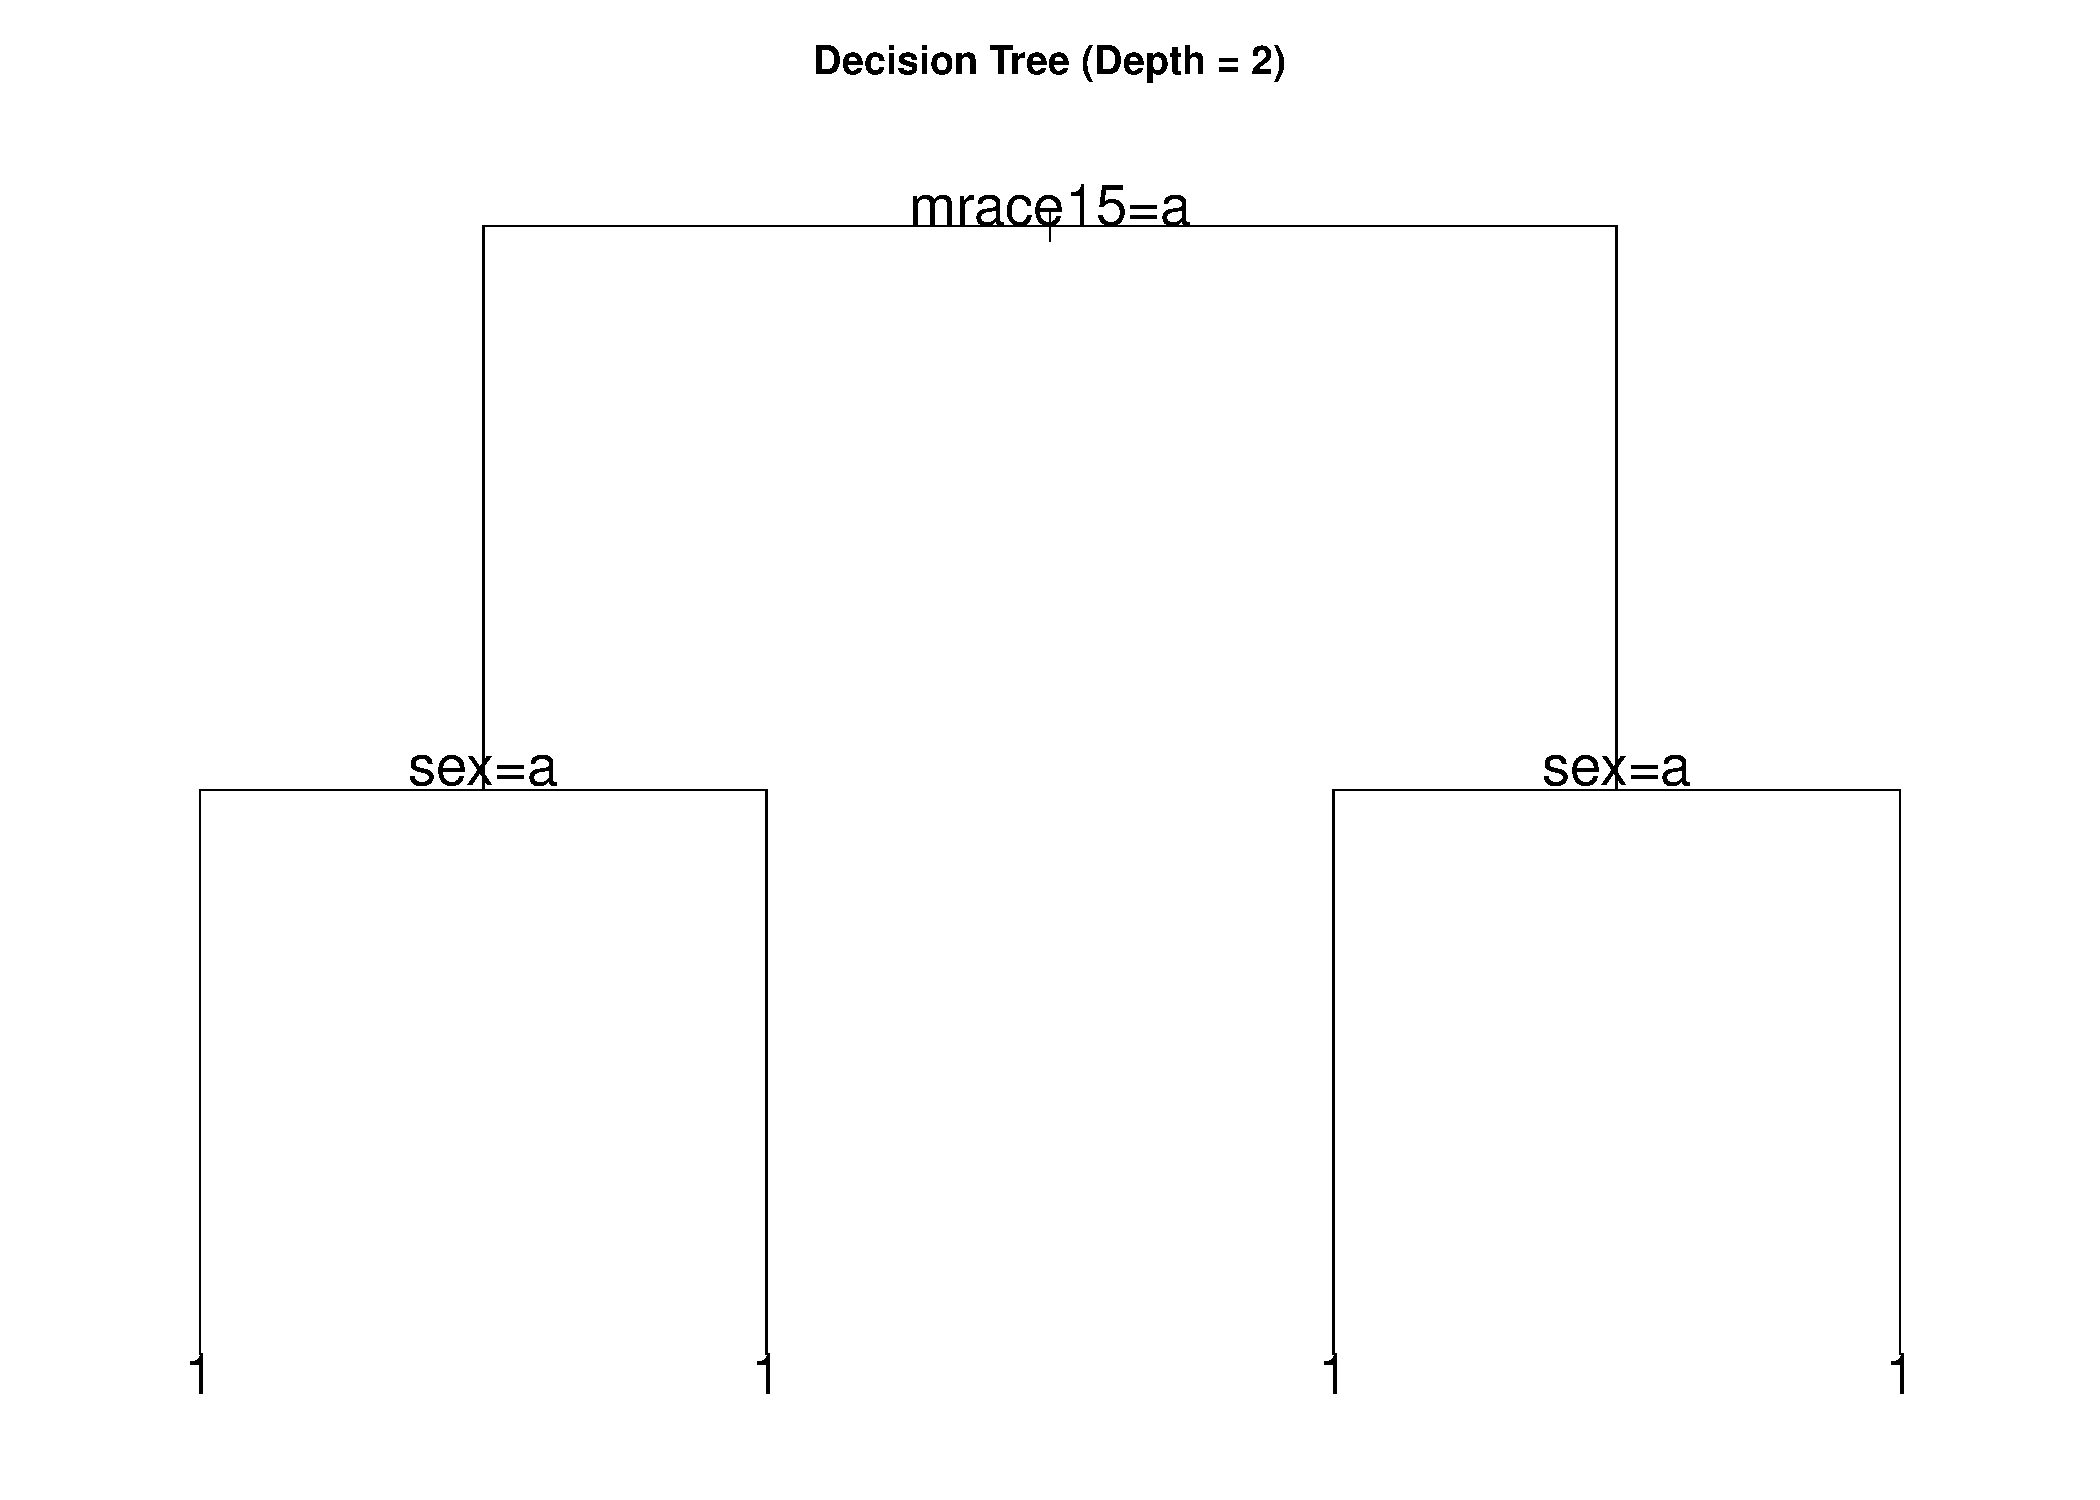
\includegraphics[width=\linewidth]{chapters/chapter3/figures/depth/plot1/decision_tree_depth_2_2021_large.pdf}
        \caption*{Maximum depth = 2}
    \end{minipage}
    \hspace{0.02\textwidth}
    \begin{minipage}{0.48\textwidth}
        \centering
        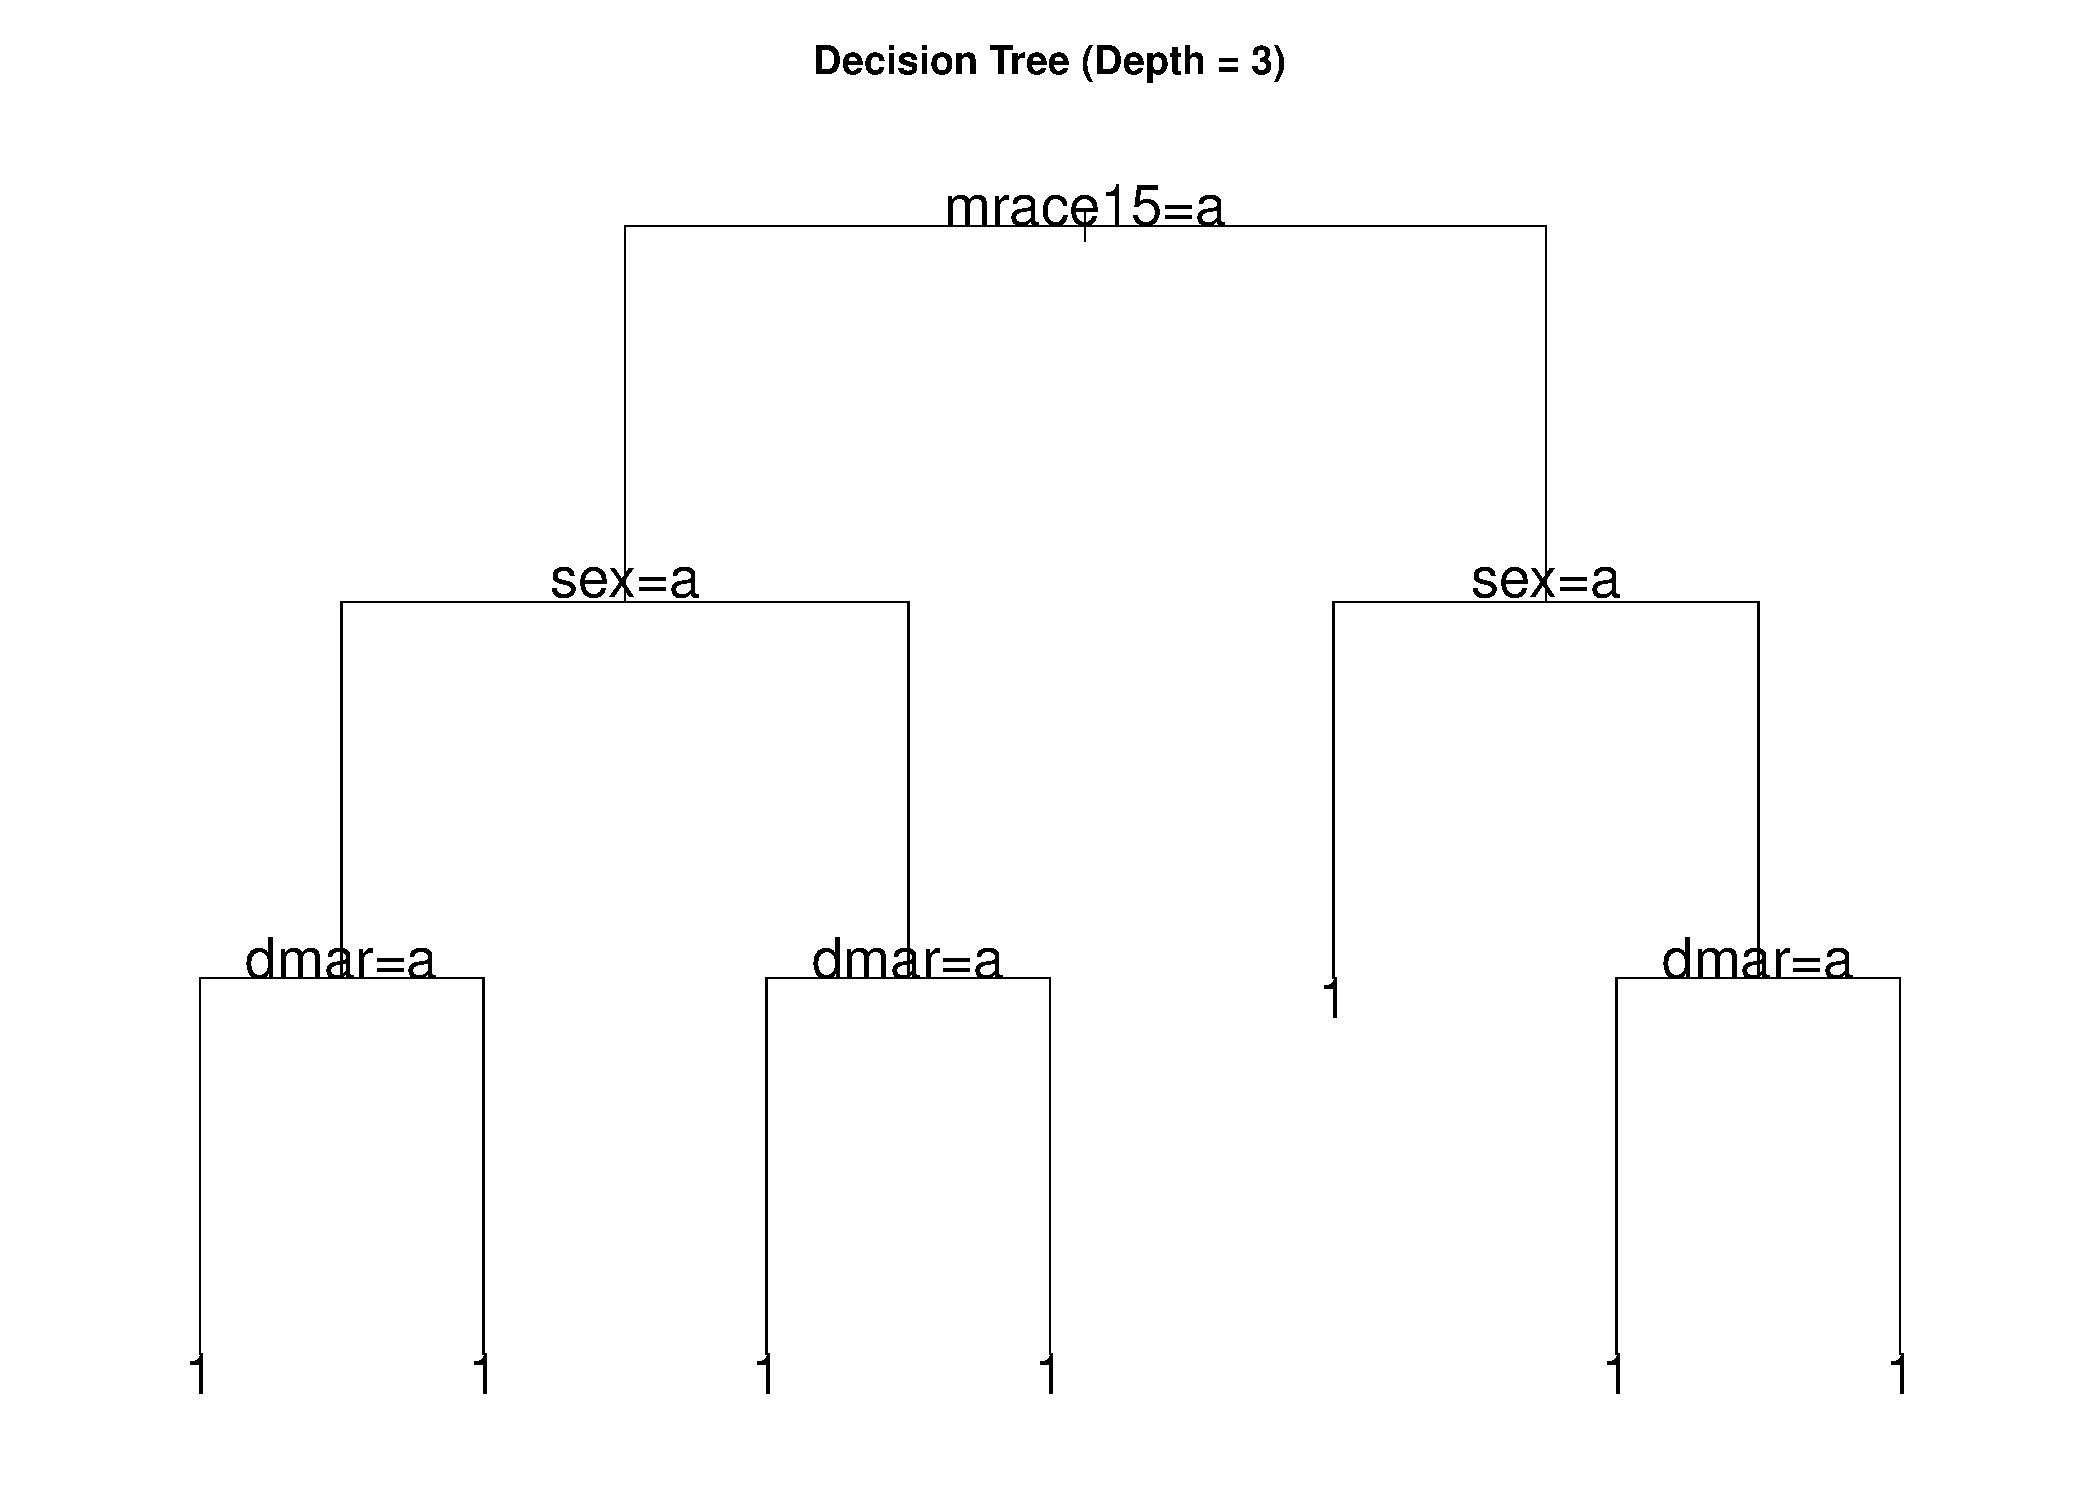
\includegraphics[width=\linewidth]{chapters/chapter3/figures/depth/plot1/decision_tree_depth_3_2021_large.pdf}
        \caption*{Maximum depth = 3}
    \end{minipage}
    
    \vspace{1cm}
    
    % Second row
    \begin{minipage}{0.48\textwidth}
        \centering
        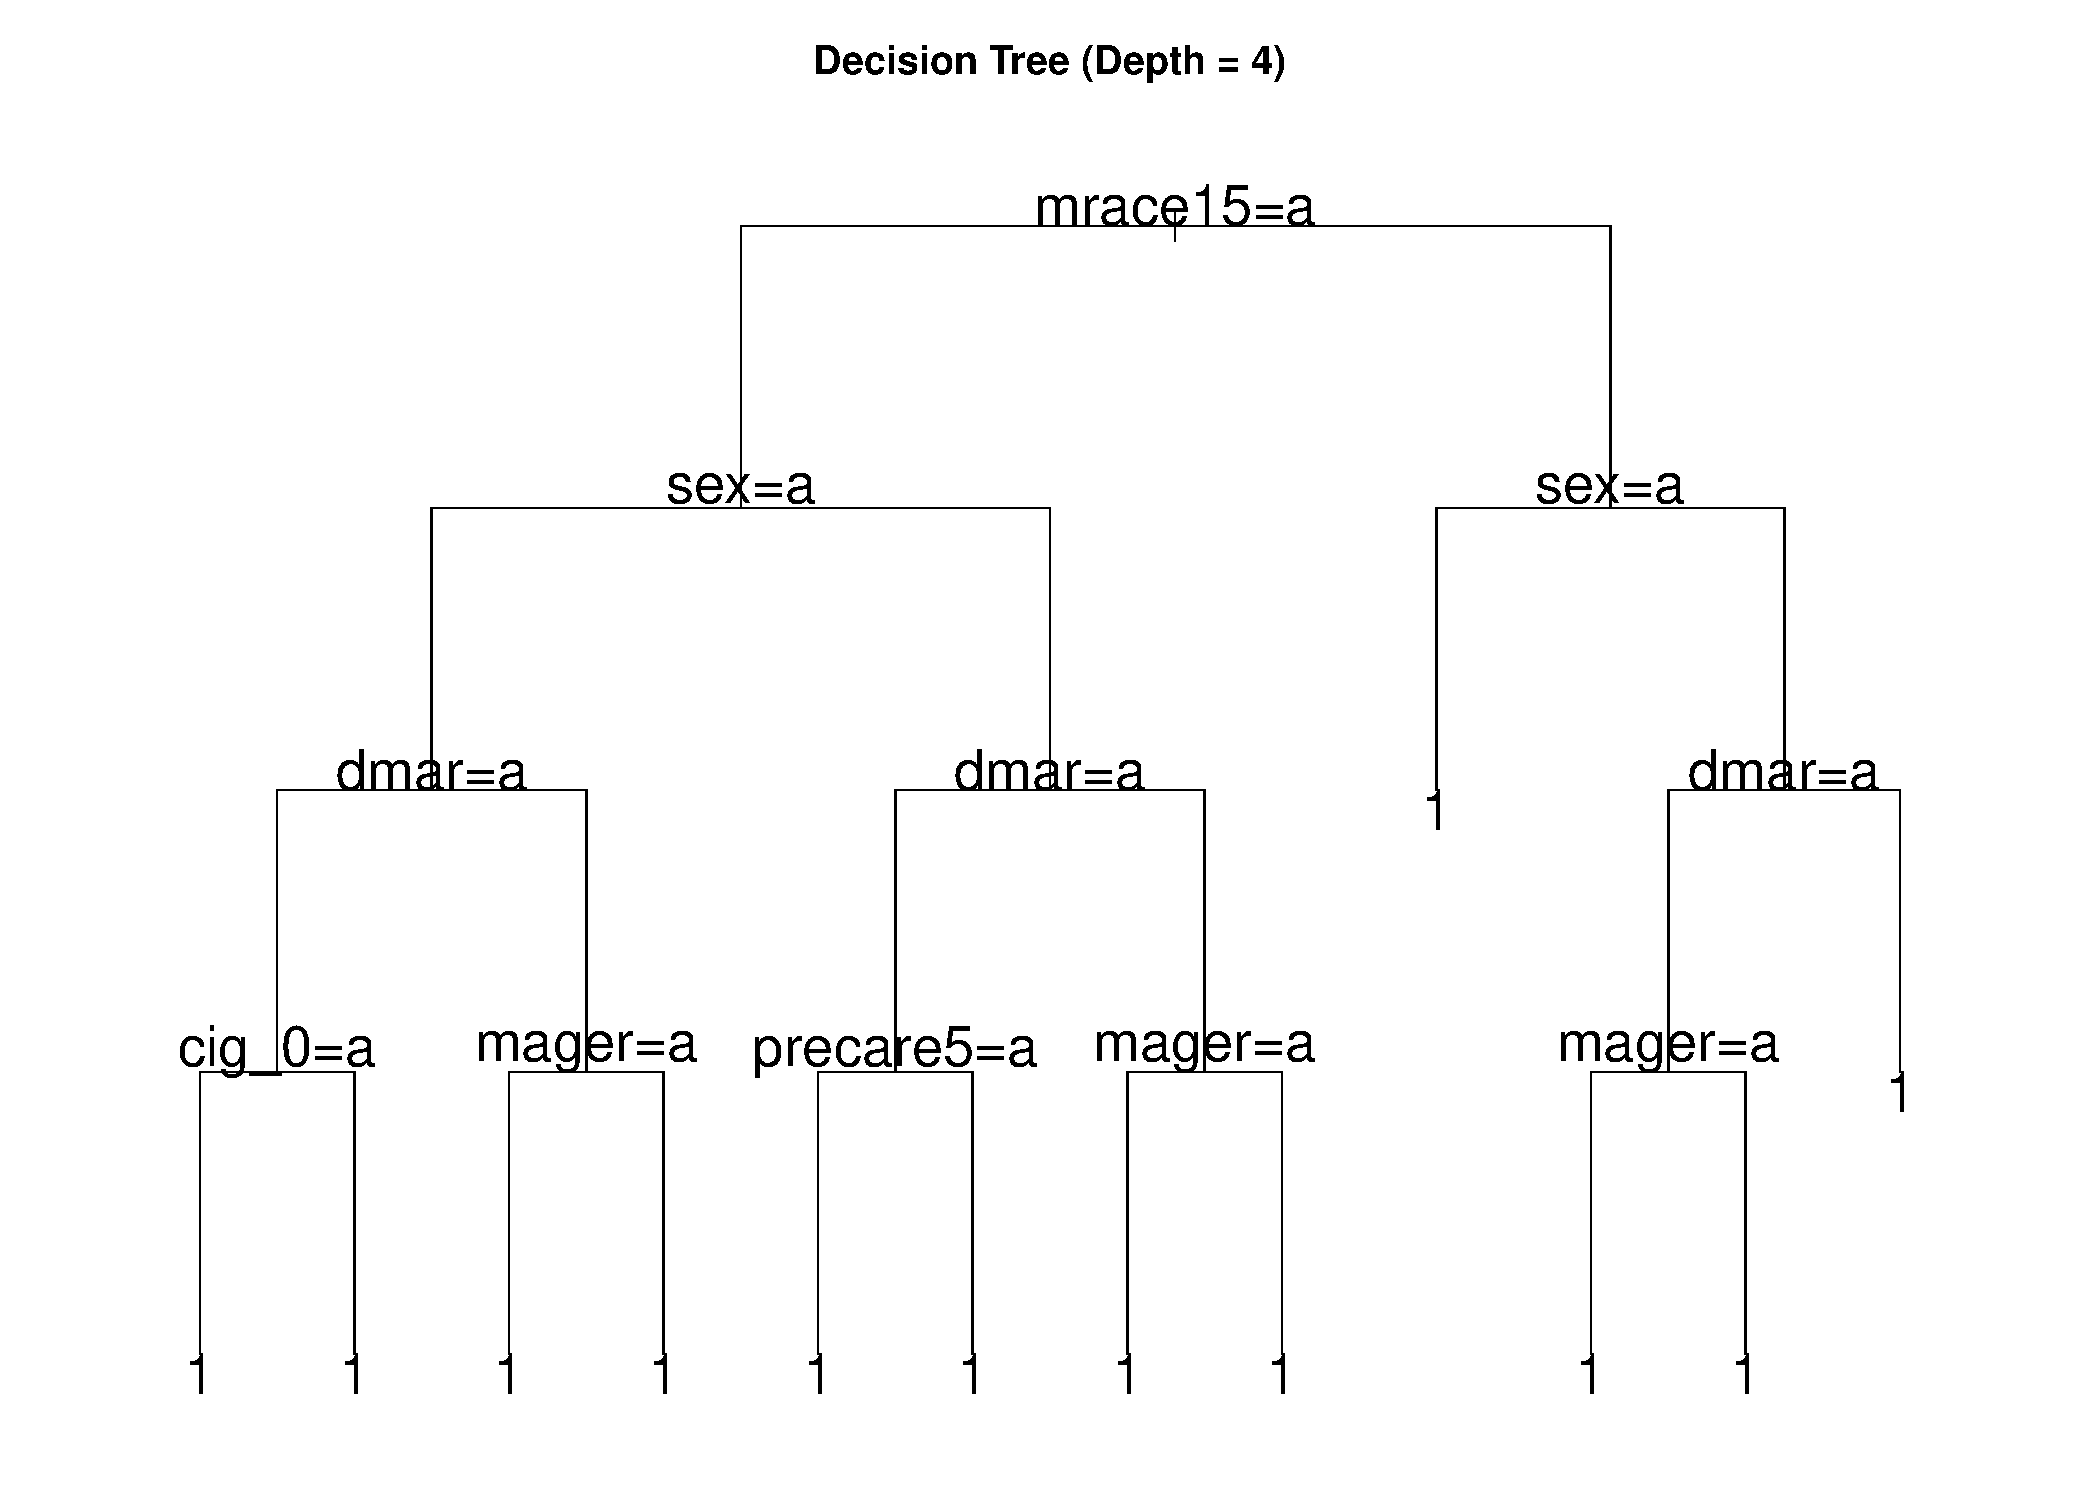
\includegraphics[width=\linewidth]{chapters/chapter3/figures/depth/plot1/decision_tree_depth_4_2021_large.pdf}
        \caption*{Maximum depth = 4}
    \end{minipage}
    \hspace{0.02\textwidth}
    \begin{minipage}{0.48\textwidth}
        \centering
        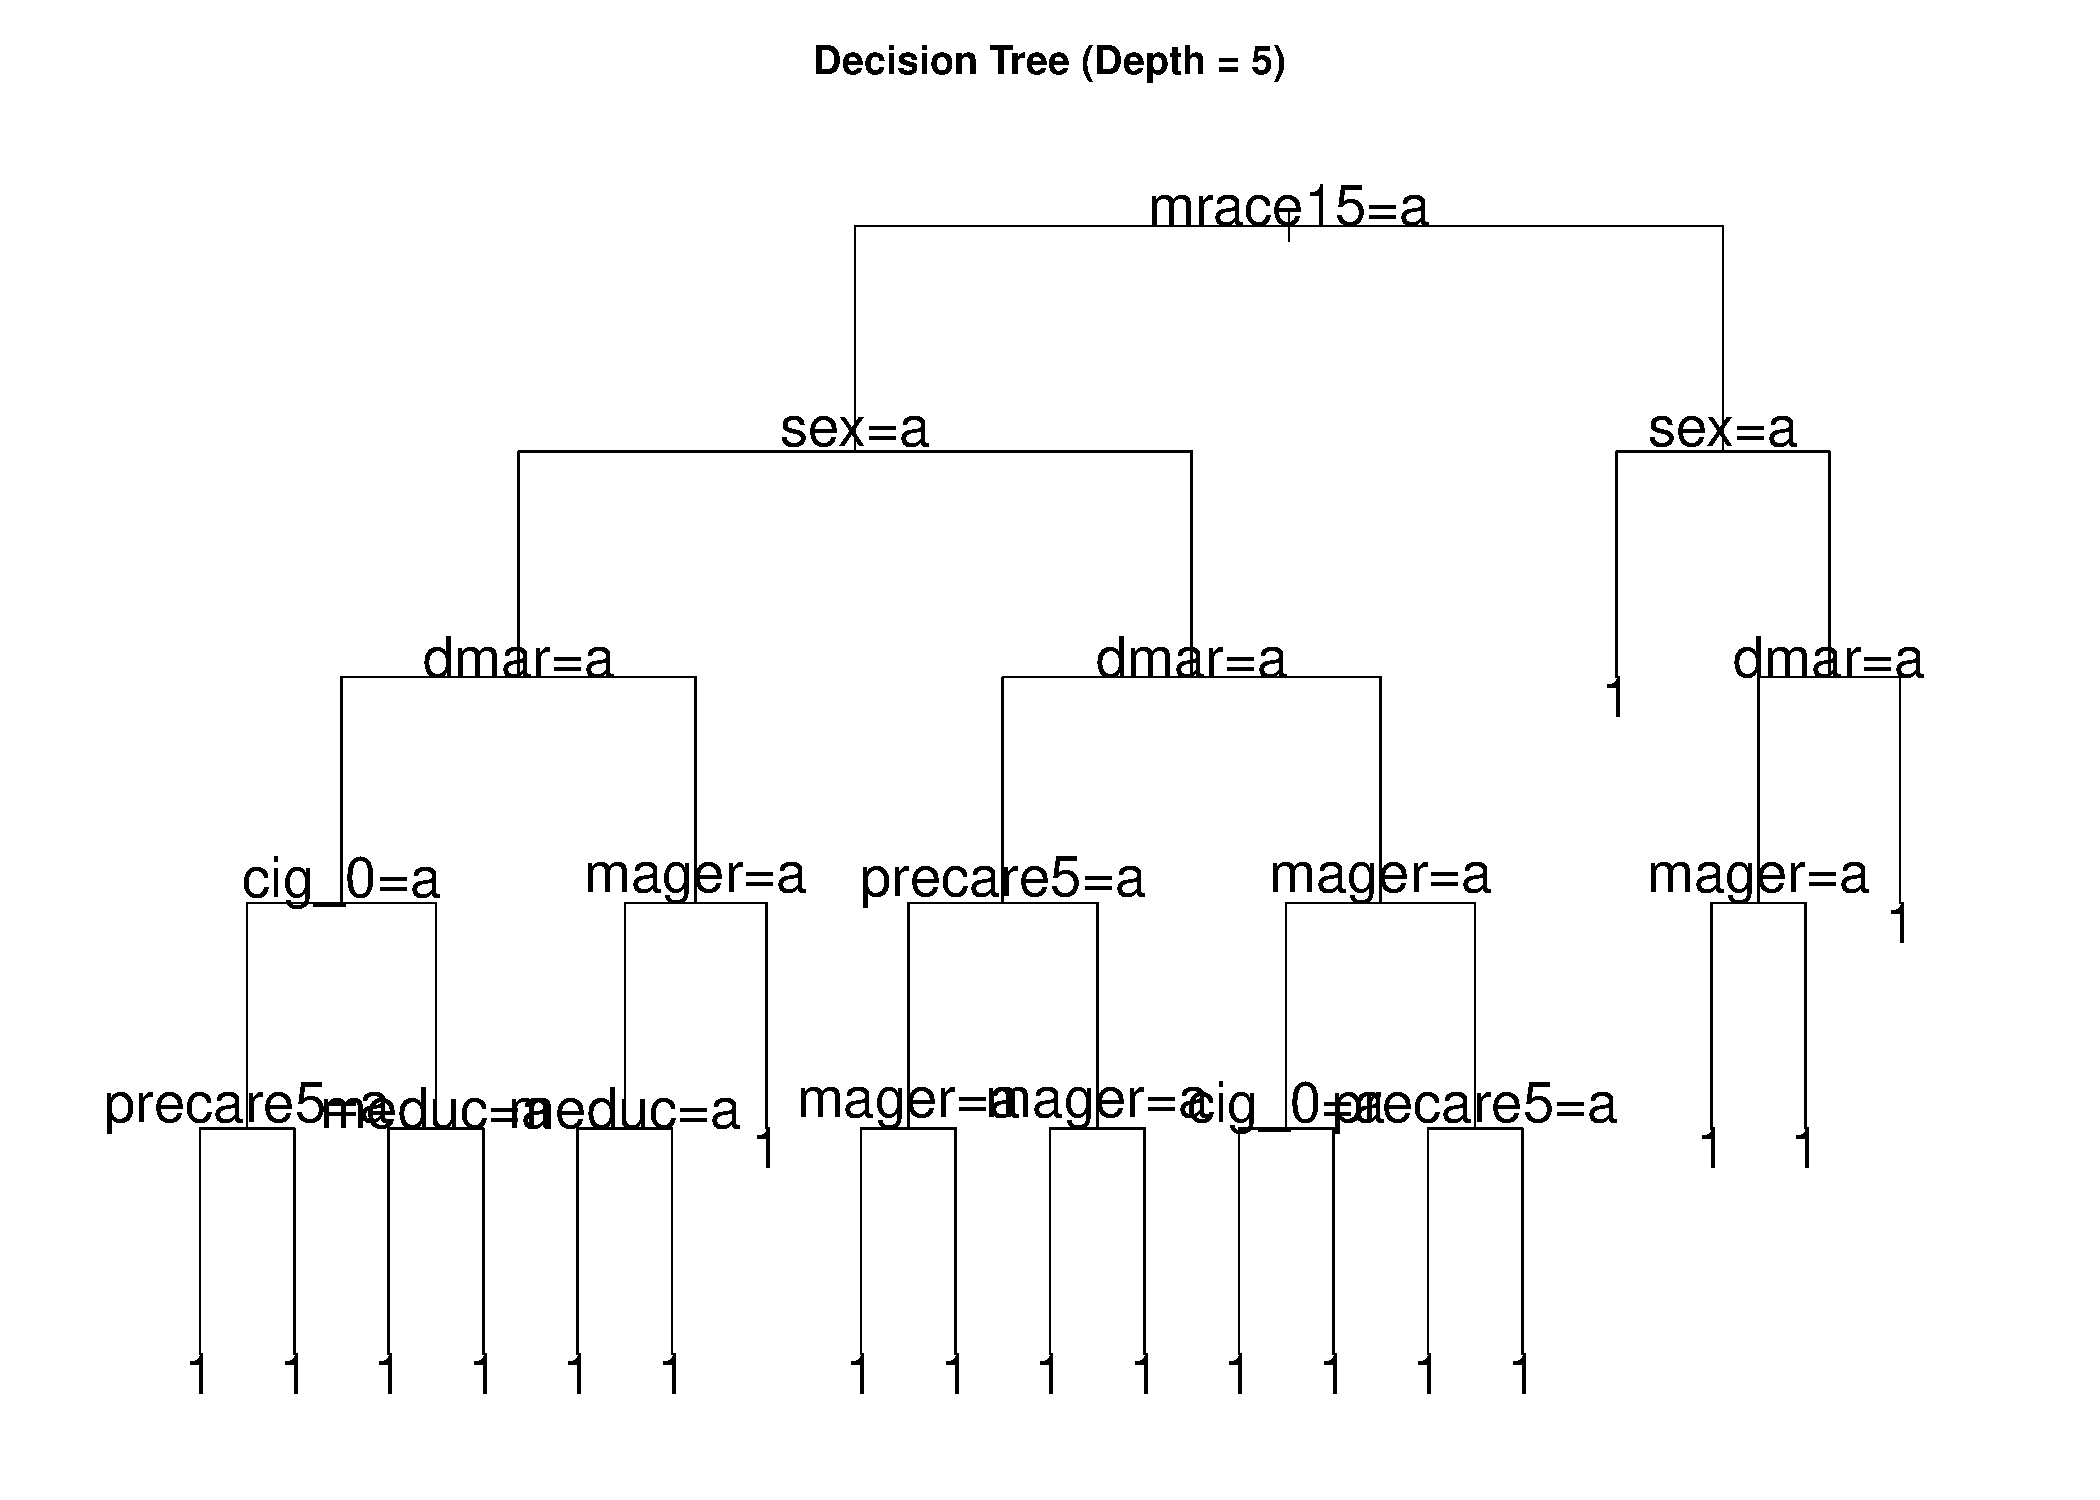
\includegraphics[width=\linewidth]{chapters/chapter3/figures/depth/plot1/decision_tree_depth_5_2021_large.pdf}
        \caption*{Maximum depth = 5}
    \end{minipage}
    \caption{Full model model tree structures showing splits at different maximum depths (2,3,4,5). The trees demonstrate variable selection patterns with increasing depth, highlighting the growing complexity of the model structure.}
    \label{fig:trees-comparison-full}
\end{figure}

% depth comparison - LBW
\begin{figure}[p]
    \centering
    % First row
    \begin{minipage}{0.48\textwidth}
        \centering
        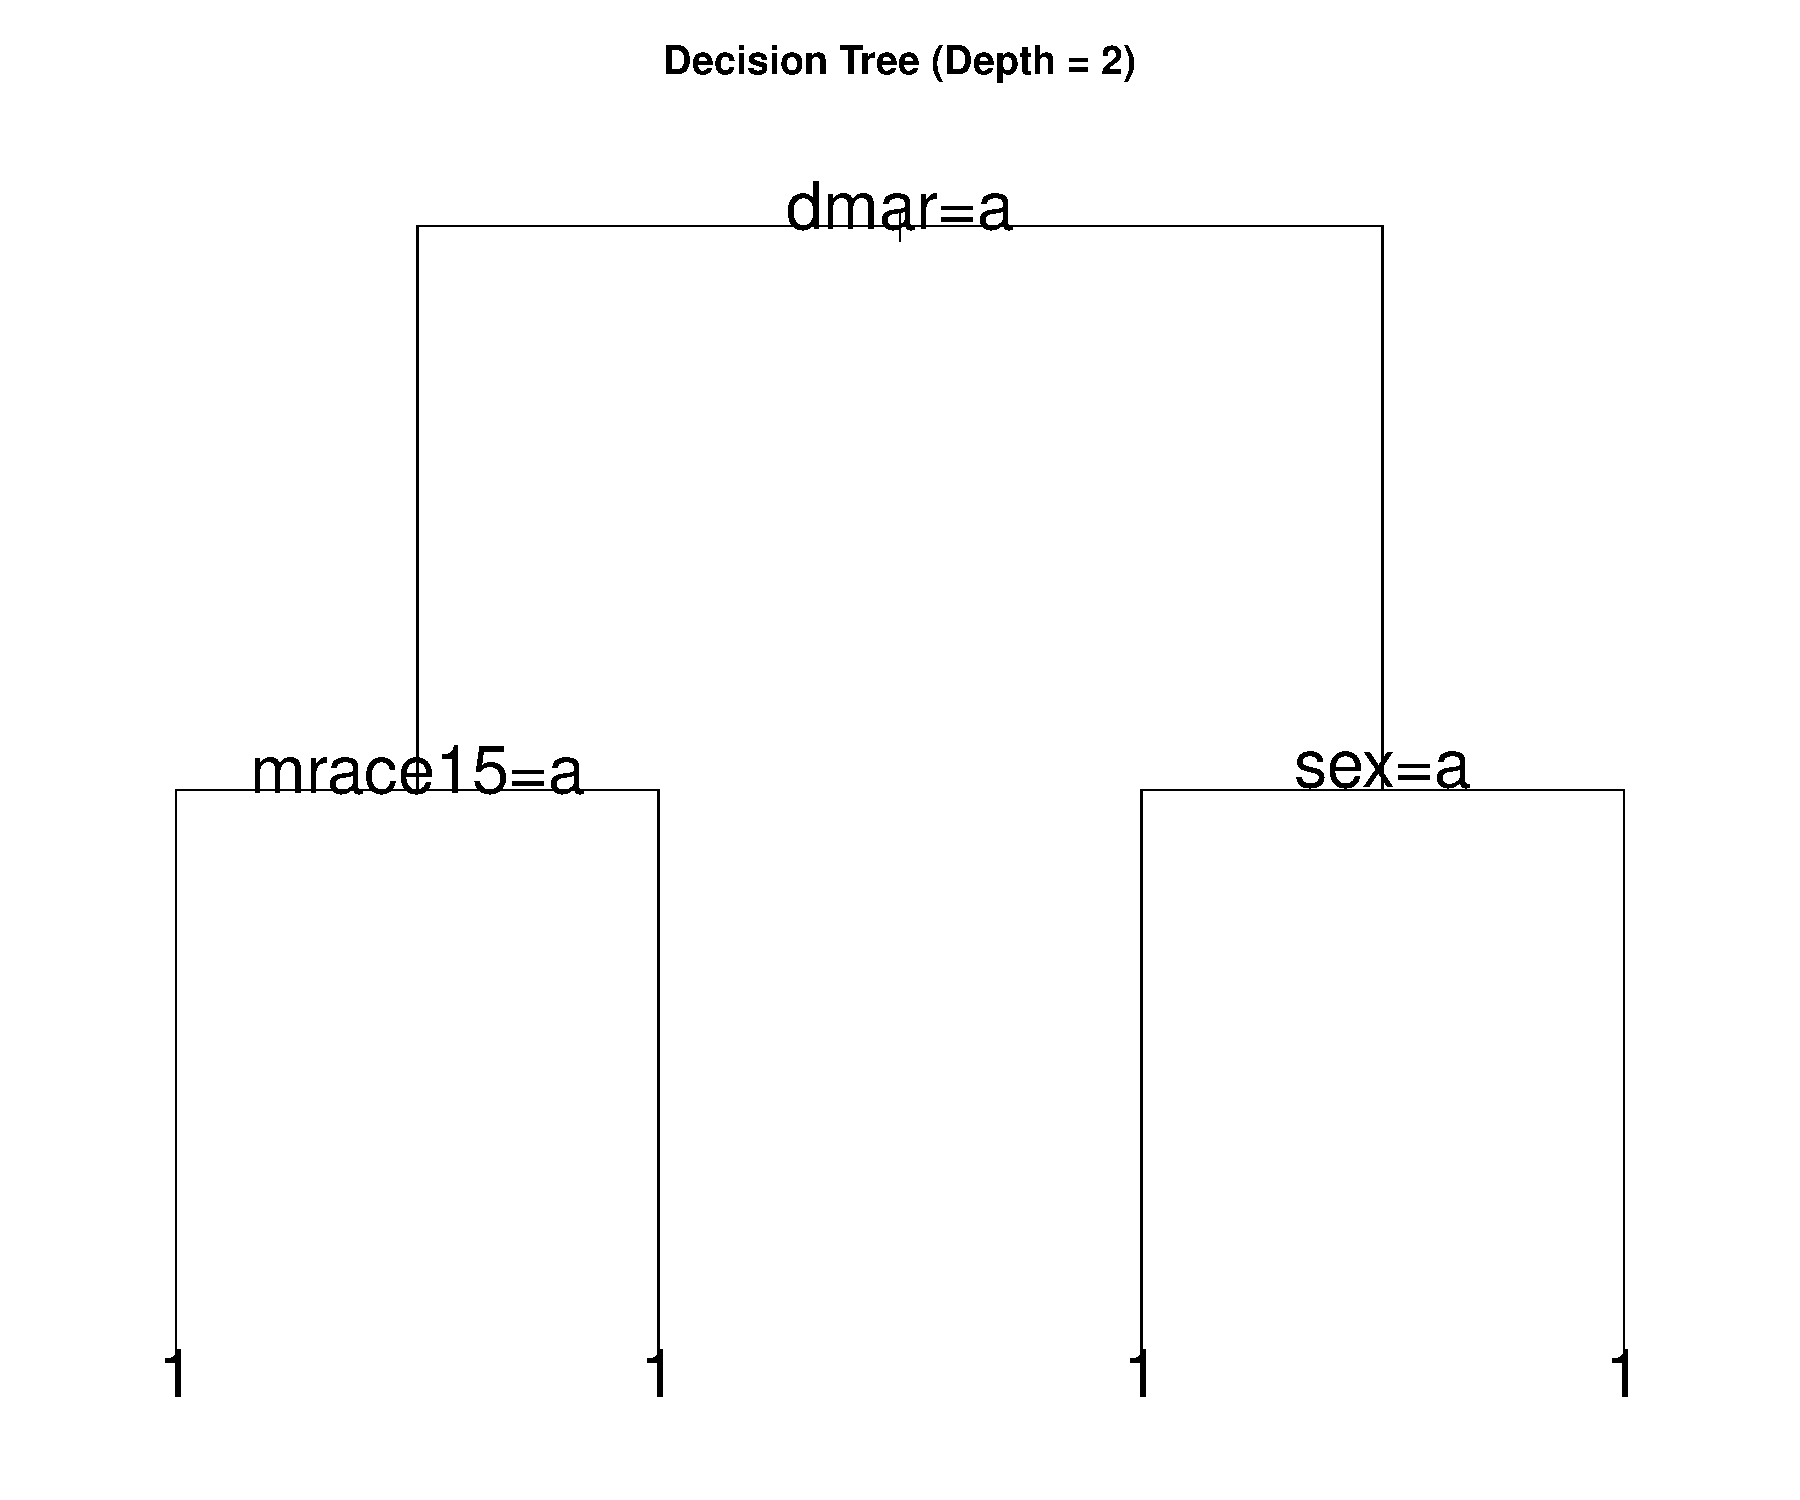
\includegraphics[width=\linewidth]{chapters/chapter3/figures/depth/plot2/decision_tree_depth_2_2021_large.pdf}
        \caption*{Maximum depth = 2}
    \end{minipage}
    \hspace{0.02\textwidth}
    \begin{minipage}{0.48\textwidth}
        \centering
        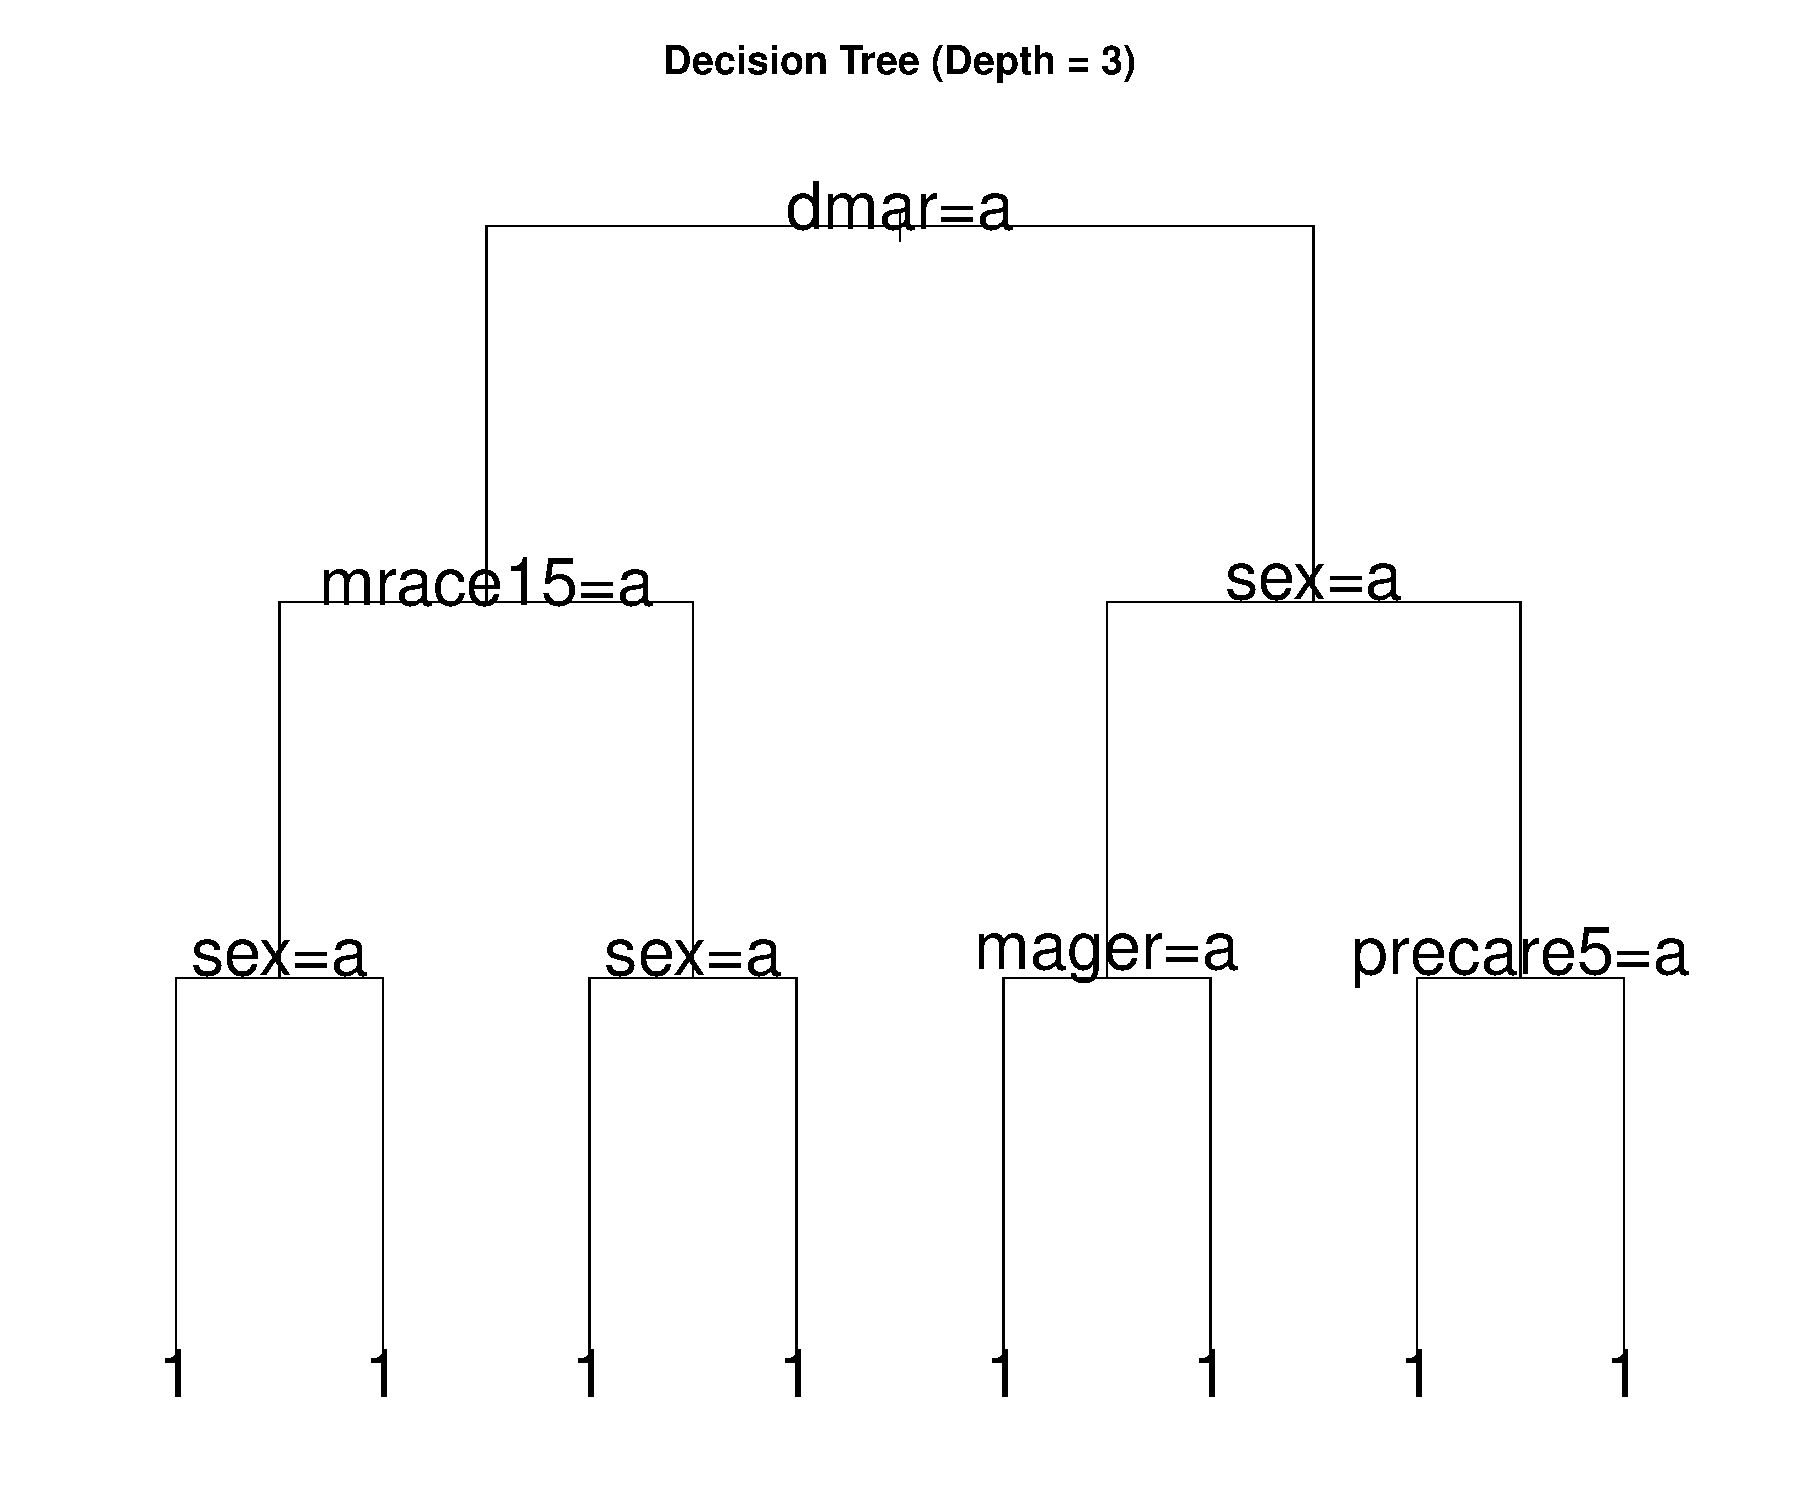
\includegraphics[width=\linewidth]{chapters/chapter3/figures/depth/plot2/decision_tree_depth_3_2021_large.pdf}
        \caption*{Maximum depth = 3}
    \end{minipage}
    
    \vspace{1cm}
    
    % Second row
    \begin{minipage}{0.48\textwidth}
        \centering
        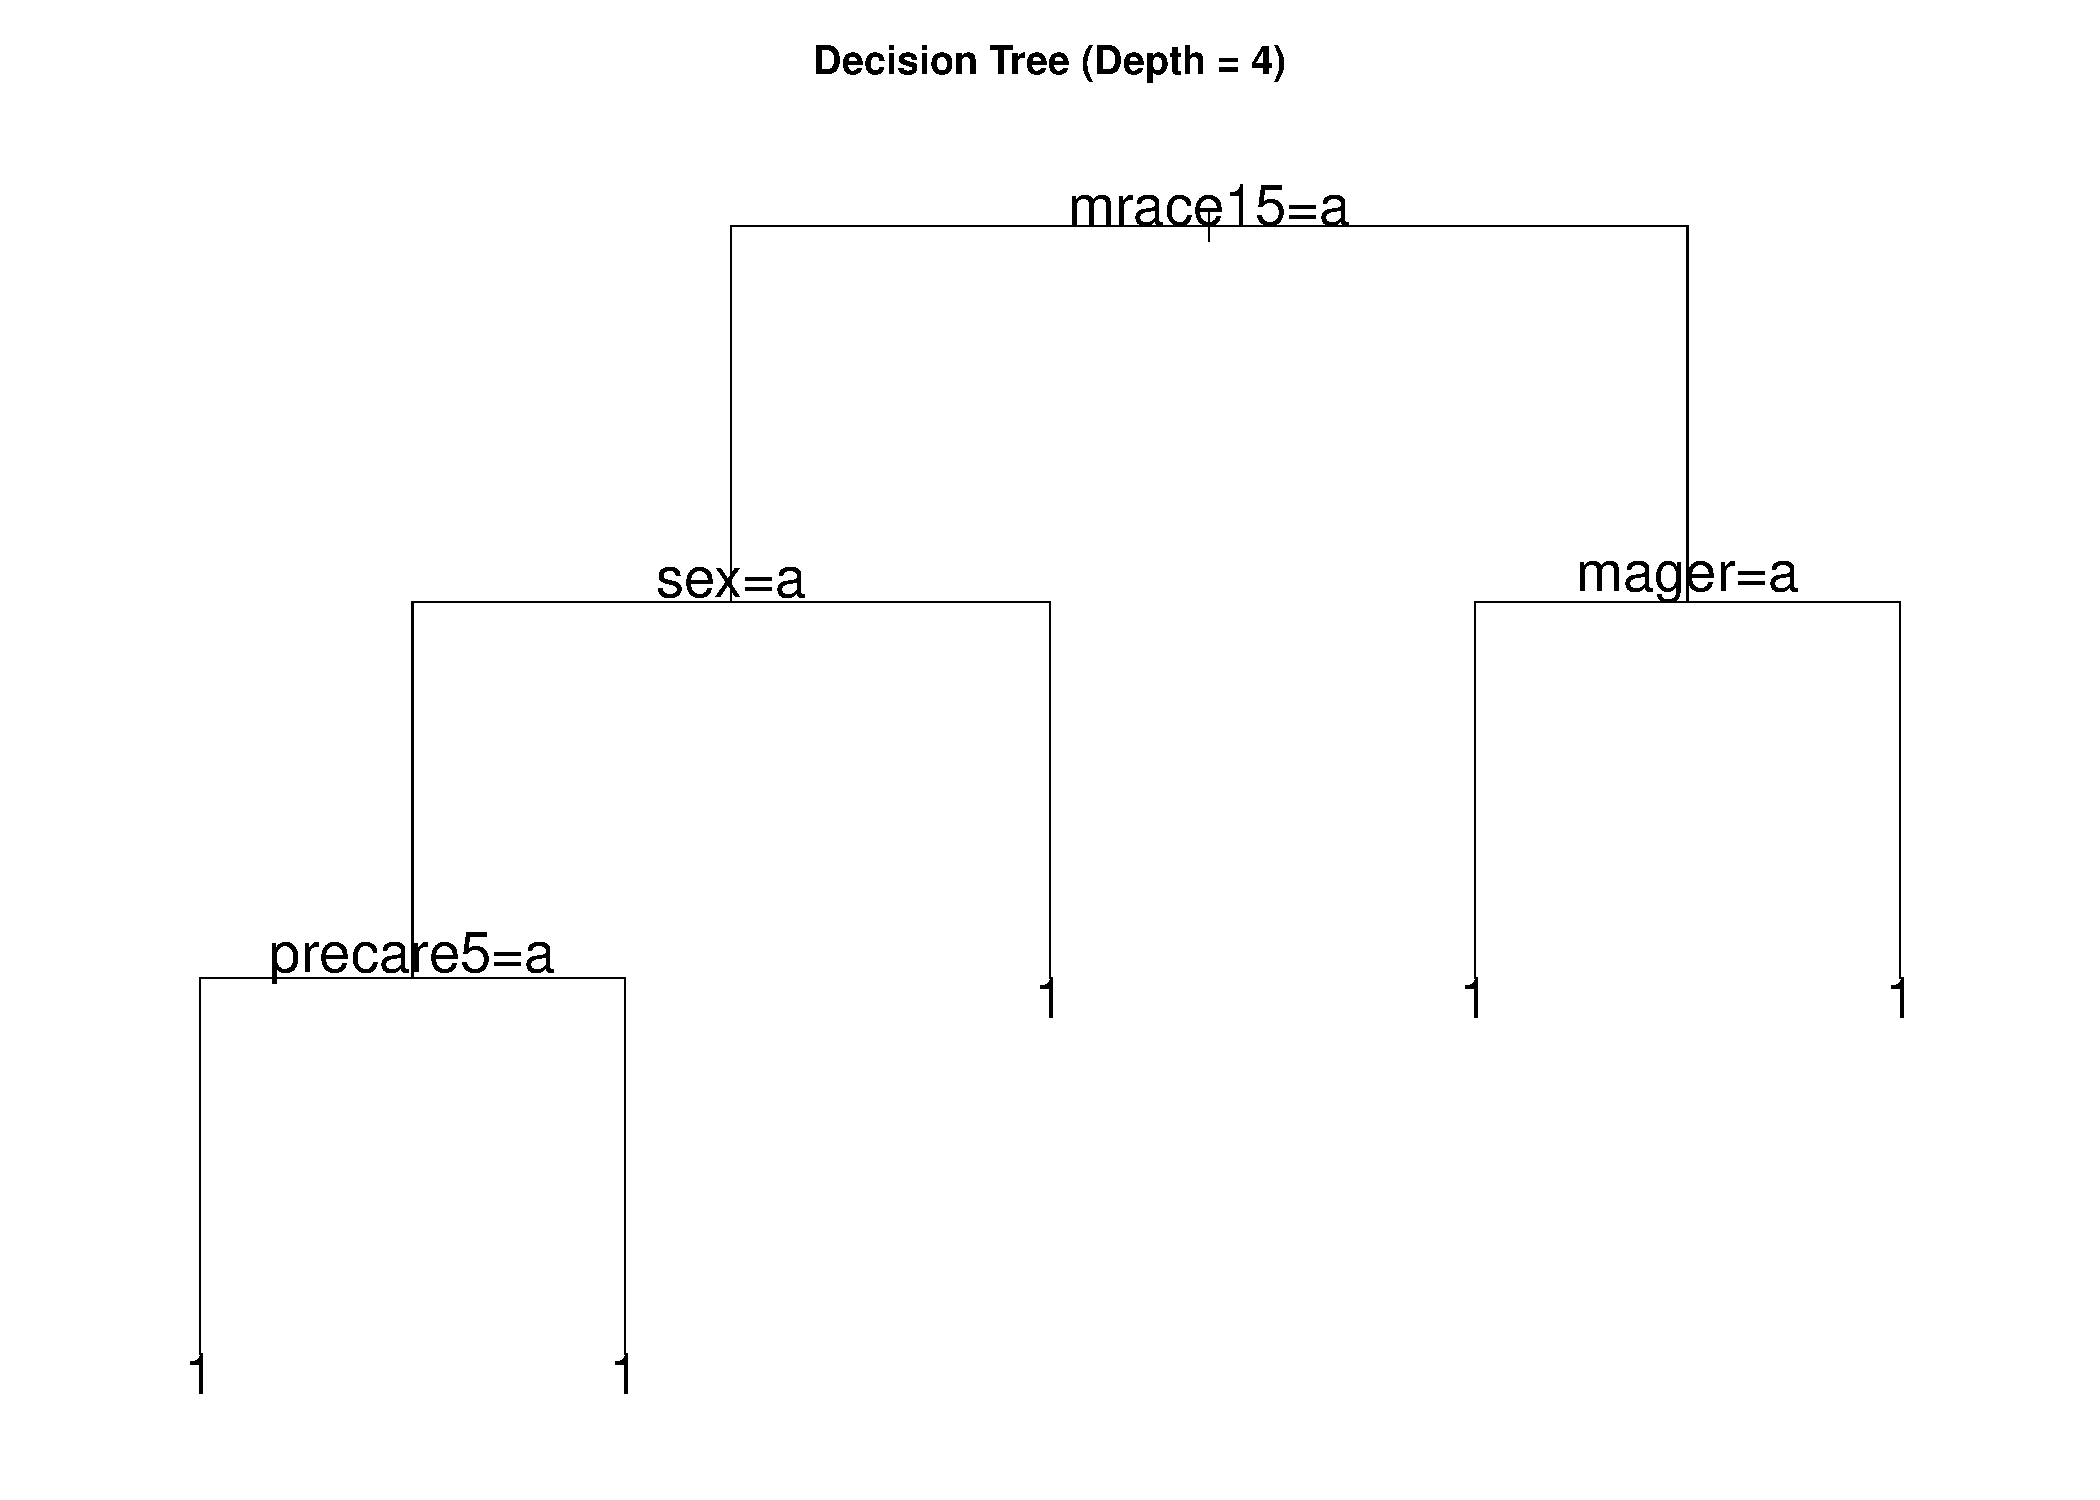
\includegraphics[width=\linewidth]{chapters/chapter3/figures/depth/plot2/decision_tree_depth_4_2021_large.pdf}
        \caption*{Maximum depth = 4}
    \end{minipage}
    \hspace{0.02\textwidth}
    \begin{minipage}{0.48\textwidth}
        \centering
        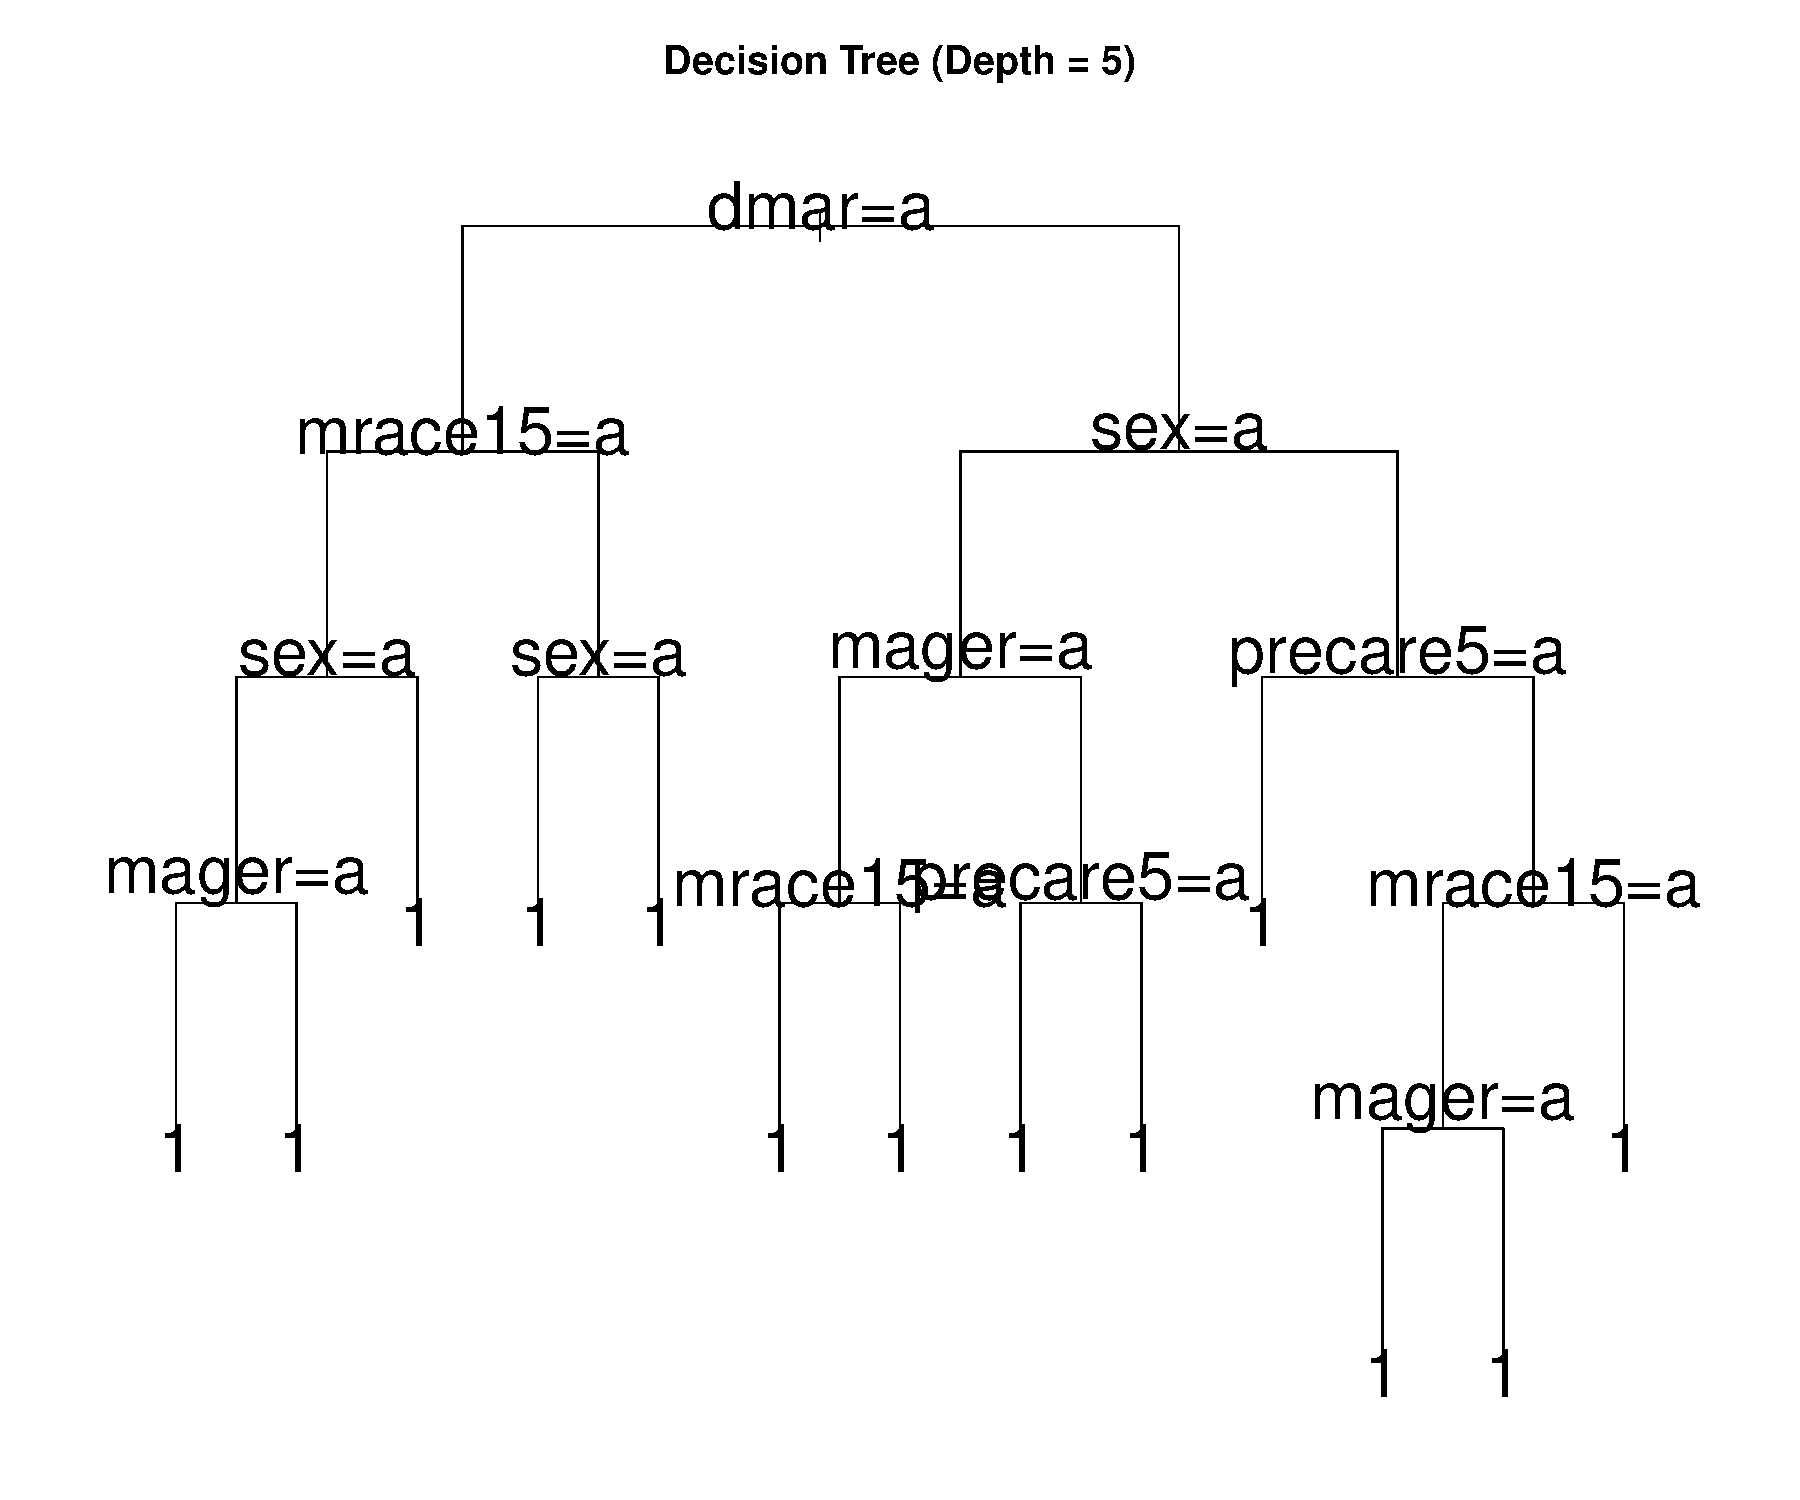
\includegraphics[width=\linewidth]{chapters/chapter3/figures/depth/plot2/decision_tree_depth_5_2021_large.pdf}
        \caption*{Maximum depth = 5}
    \end{minipage}
    \caption{LBW-only model tree structures showing splits at different maximum depths (2,3,4,5). The trees demonstrate variable selection patterns with increasing depth, highlighting the growing complexity of the model structure.}
    \label{fig:trees-comparison-lbw}
\end{figure}


% First barplot figure
\begin{figure}
    \centering
    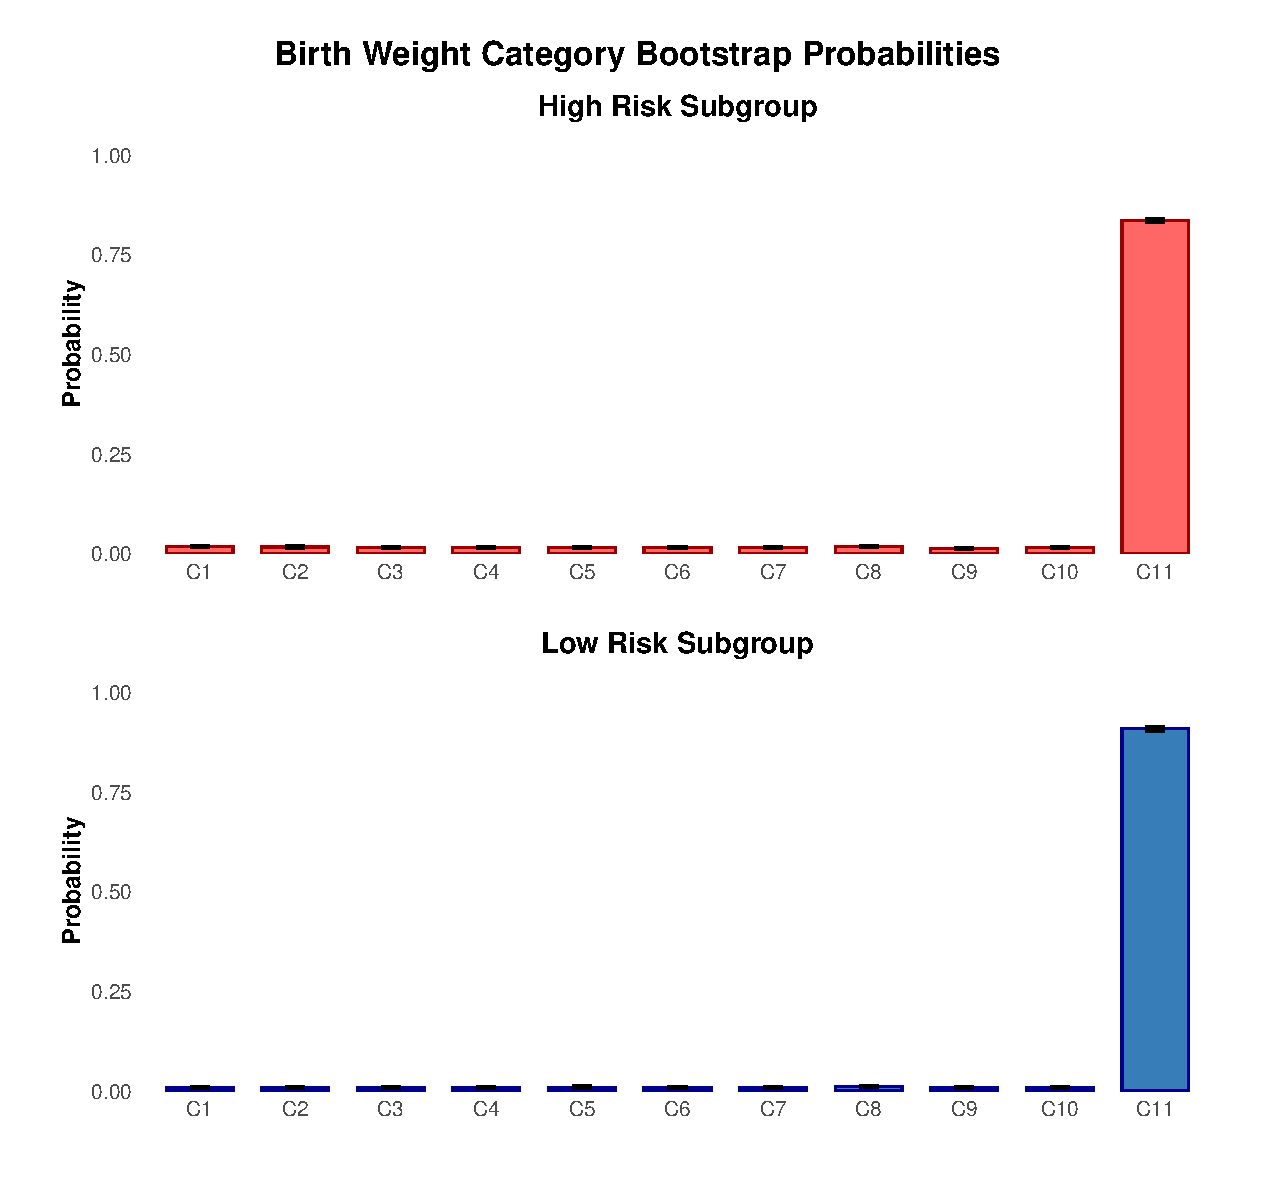
\includegraphics[width=1\textwidth]{chapters/chapter3/figures/high_low_risk_full.pdf}
    \caption{Full model: Aggregated mean probability estimates by birth weight category across $B$ bootstraps, showing the distribution of predicted probabilities for high and low risk subgroups with 95\% confidence intervals.}
    \label{fig:high-low-risk-full}
\end{figure}

% Second barplot figure
\begin{figure}
    \centering
    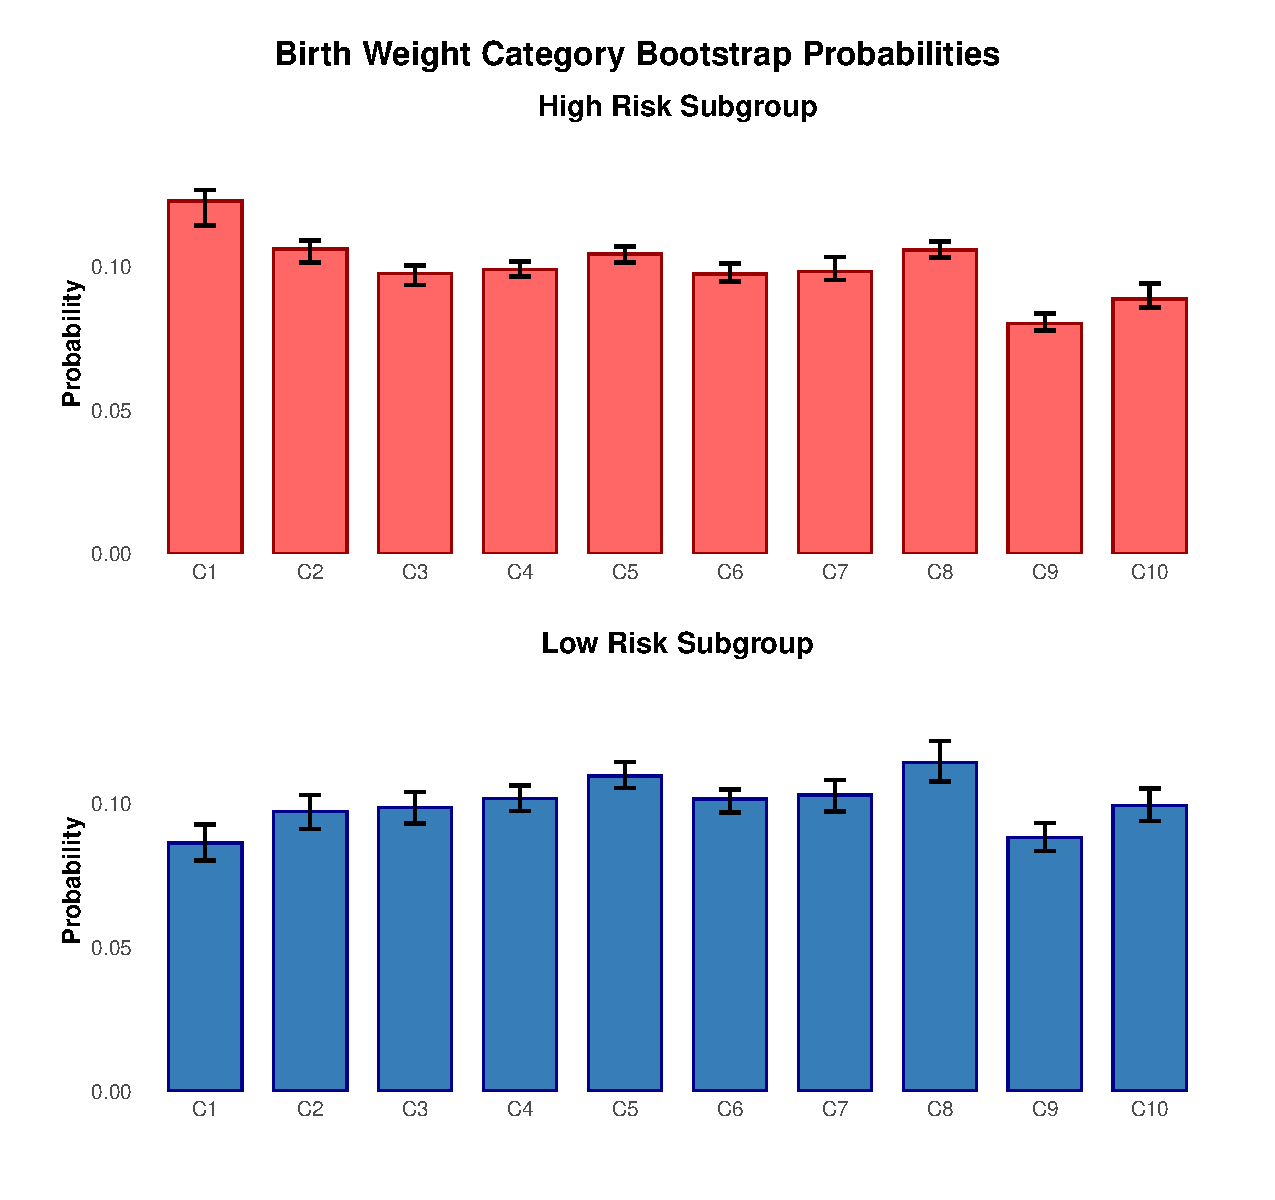
\includegraphics[width=1\textwidth]{chapters/chapter3/figures/high_low_risk_small.pdf}
    \caption{LBW-only model: Aggregated mean probability estimates by birth weight category across $B$ bootstraps, showing the distribution of predicted probabilities for high and low risk subgroups with 95\% confidence intervals.}
    \label{fig:high-low-risk-lbw}
\end{figure}


% Depth distributions — Full model
\begin{figure}[htbp]
    \centering
    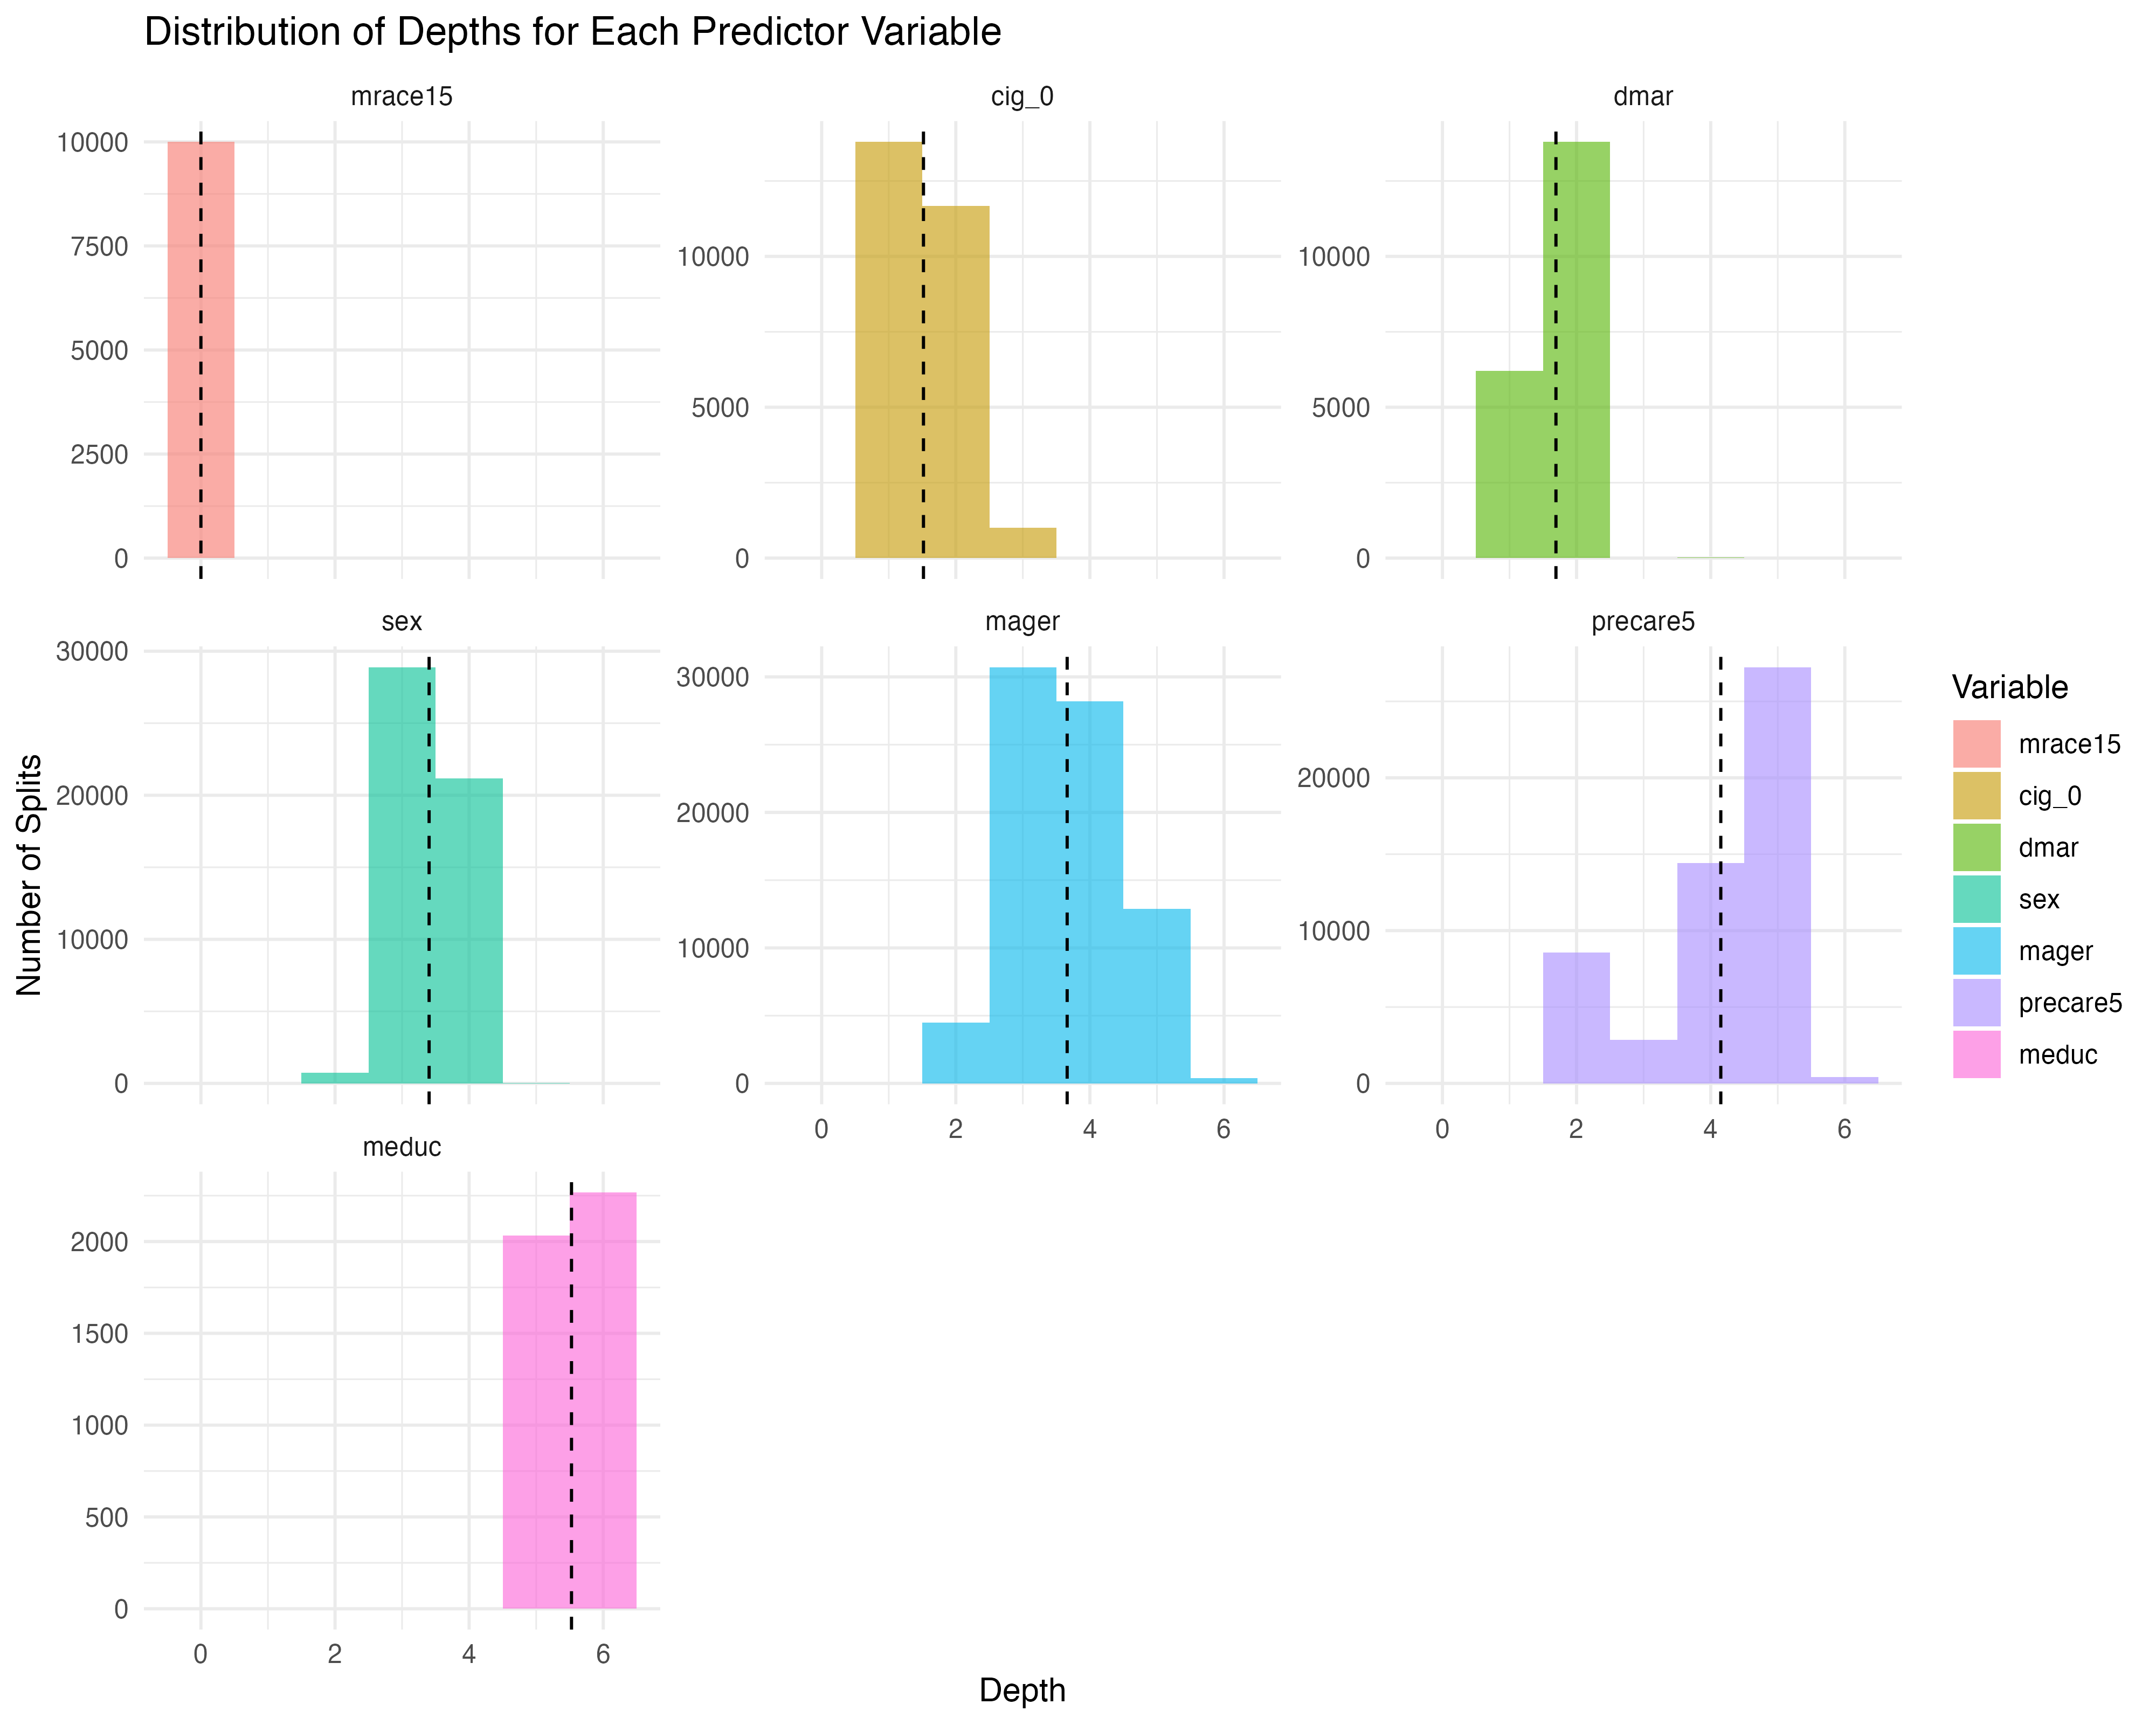
\includegraphics[width=1.0\textwidth]{chapters/chapter3/figures/boot/depth_distributions.png}
    \caption{Full model: Distribution of variable depths across the ensemble. Each panel shows a histogram indicating how frequently a given variable appears at each tree depth, where depth 0 corresponds to the root node. Variables closer to the root are generally more important in the model.}
    \label{fig:var-depth-distributions-full}
\end{figure}

% Depth distributions — LBW-only model
\begin{figure}[htbp]
    \centering
    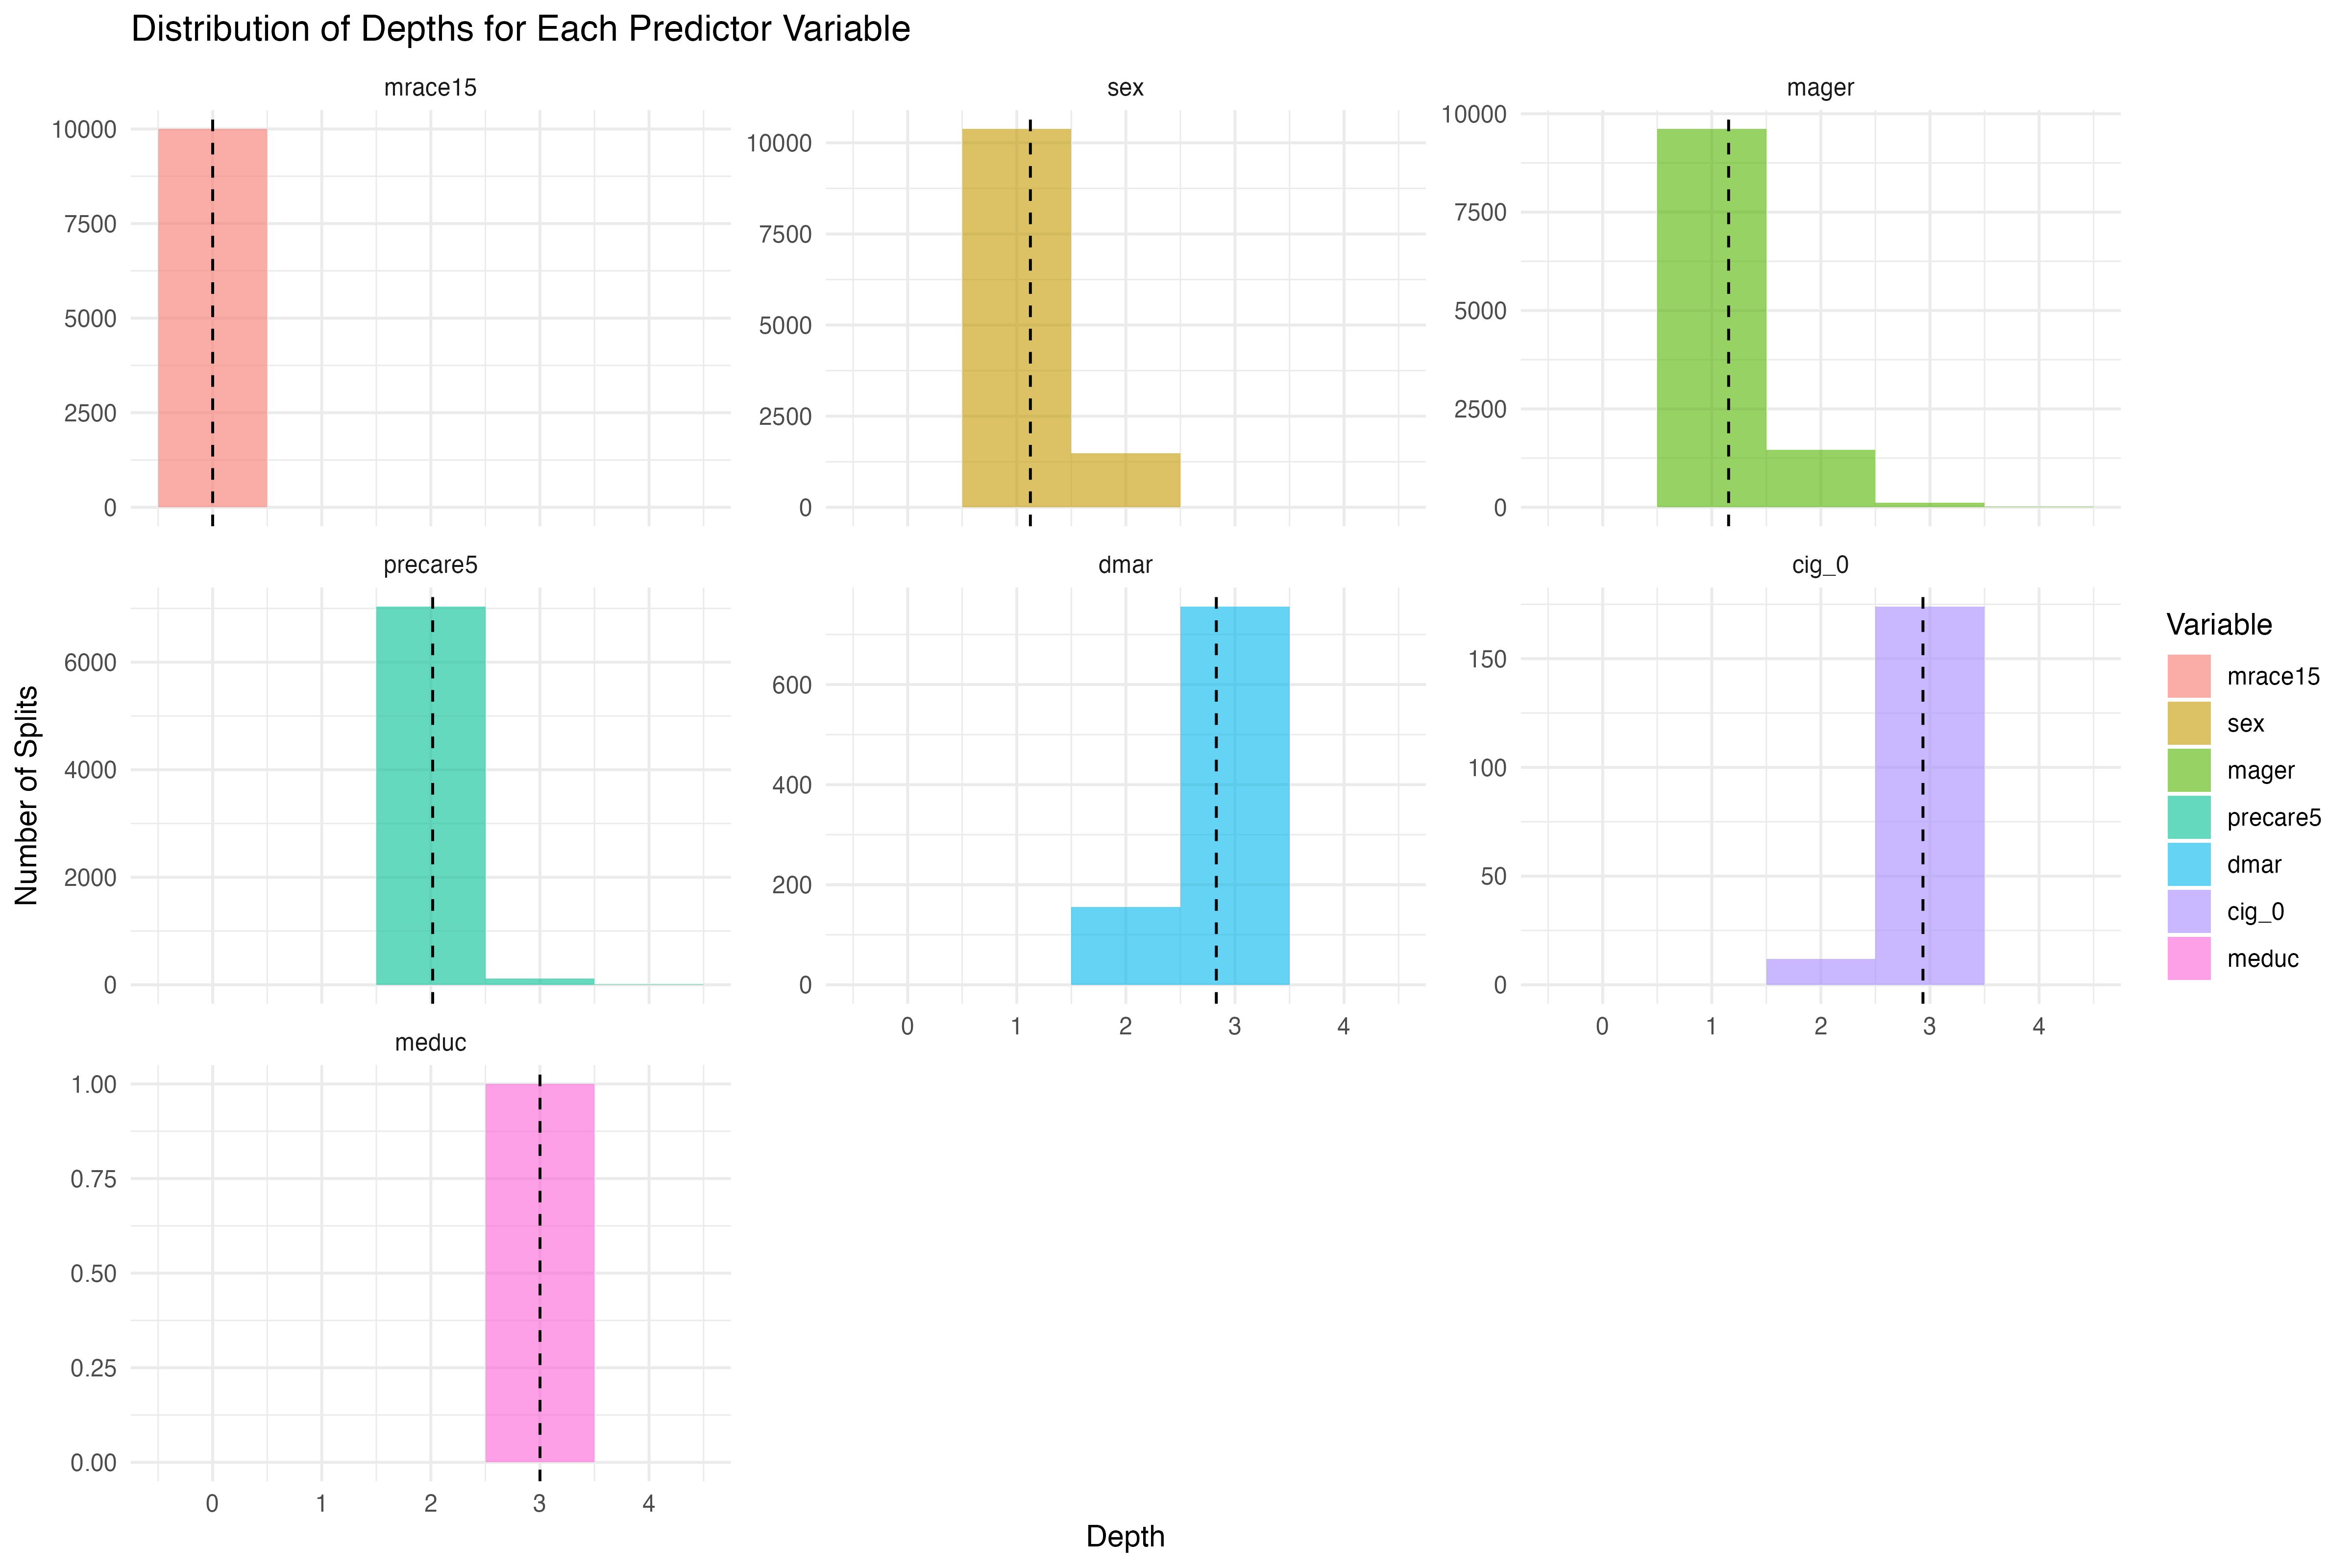
\includegraphics[width=1.0\textwidth]{chapters/chapter3/figures/boot/depth_distributions_2.png}
        \caption{LBW-only model: Distribution of variable depths across the ensemble. Each panel shows a histogram indicating how frequently a given variable appears at each tree depth, where depth 0 corresponds to the root node. Variables closer to the root are generally more important in the model.}
    \label{fig:var-depth-distributions-lbw}
\end{figure}

